\documentclass[a4paper,12pt]{article}
\usepackage{graphicx}
\graphicspath{ {../images/} }
\usepackage{float}
\renewcommand\thesection{\arabic{section}}
\newcommand{\tab}[1]{\hspace{.1\textwidth}\rlap{#1}}

\begin{document}
	
\begin{titlepage}
	\newcommand{\HRule}{\rule{\linewidth}{0.5mm}} % Defines a new command for the horizontal lines, change thickness here

	\center % Center everything on the page
	 
	
	%----------------------------------------------------------------------------------------
	%	TITLE SECTION
	%----------------------------------------------------------------------------------------

	
	{ \huge \bfseries Application Requirements and Design}\\\HRule \\[0.4cm] % Title of your document
	\Large \textbf{Real-time Geospatial Data Processor and Visualiser} \\
	\small \emph{\textbf{Client: Werner Raath}}
	\HRule \\[1.5cm]
	 
	%----------------------------------------------------------------------------------------
	%	MEMBERS, TEAM NAME SECTION
	%----------------------------------------------------------------------------------------
	
\includegraphics[width=\textwidth]{name} \\[1cm]
	\begin{minipage}{0.4\textwidth}
	\begin{flushleft} \large
	
\includegraphics[width=\textwidth]{logo} \\[0.5cm]
	{\large 7 October 2016}\\
	{\large v0.4}
	\end{flushleft}
	\end{minipage}
	~
	\begin{minipage}{0.5\textwidth}
	\begin{flushright} \large
	\emph{Members:}\\% add your name
	Nsovo Baloyi 12163262

	Maluleki Nyuswa 13040686
	
	Keletso Molefe 14222583
	
	Kamogelo Tswene 12163555

	\end{flushright}
	\end{minipage}\\[4cm]
\end{titlepage}


	\newpage
	
	%-------------------------------------------------------------------------------------
	%		TABLE OF CONTENTS
	%-------------------------------------------------------------------------------------
	\tableofcontents
	\newpage
	\section*{Document History}
	\addcontentsline{toc}{section}{\protect\numberline{}Document History}
	
	\begin{table}[h!]
		
		\centering % used for centering table
		\begin{tabular}{c c c c} % centered columns (4 columns)
			\hline\hline %inserts double horizontal lines
			Version & Date & Changed By & Summary \\ [0.5ex] % inserts table
			%heading
			\hline % inserts single horizontal line
			v0.1 & 27 May 2016 	& Nsovo Baloyi 		& First Draft 
			\\ & 				& Maluleki Nyuswa 	&  
			\\ & 				& Keletso Molefe 	&
			\\ & 				& Kamogelo Tswene 	& \\ [1ex] 
			\hline
			v0.2 & 29 July 2016 & Maluleki Nyuswa	& Second Draft
			\\ & 				& Kamogelo Tswene 	  
			\\ & 				& 	&
			\\ & 				&  	& \\ [1ex] 
			\hline % inserts single horizontal line
			v0.3 & 9 September 2016 	& Nsovo Baloyi 		& Third Draft 
			\\ & 				& Maluleki Nyuswa 	&  
			\\ & 				& Keletso Molefe 	&
			\\ & 				& Kamogelo Tswene 	& \\ [1ex] 
			\hline % inserts single horizontal line
			v0.4 & 7 October 2016 	& Nsovo Baloyi 		& Fourth Draft 
			\\ & 				& Maluleki Nyuswa 	&  
			\\ & 				& Keletso Molefe 	&
			\\ & 				& Kamogelo Tswene 	& \\ [1ex] 
			\hline\hline
		\end{tabular}
		\label{table:nonlin} % is used to refer this table in the text
	\end{table}

	\newpage
	
	%-------------------------------------------------------------------------------------
	%		INTRODUCTION
	%-------------------------------------------------------------------------------------
	\section{Introduction}	
	This documentation is the testing documentation for the Geospatial Data Processor and Visualiser project. It outlines the entire testing plan and it documentation process. The documentation firstly establishes the scope, thereafter the testing environment is discussed including all the relevant assumptions and dependencies made during the testing process. The test items, functional features that were tested and the individual test cases are then discussed. Test conducted are then specified according to whether they passed or failed. Test deliverables are then clearly tabulated followed by detailed test results, and finally conclusions and recommendations are noted.

\subsection{Purpose}

This document combines the unit test plan and report into a single coherent artefact. The Geospatial Data Processor and Visualiser system aims to collects geospatial data from third party API's, persist the data on a database and thereafter visualise such in real-time through a web-interface. The system focuses mainly on natural disaster and weather visualisation. 


Software testing forms an integral part of software design, intended to empirically verify whether the software being developed conforms to specifications. Unit testing test a piece of code in isolation against requirements and when done constructively it contributes to code flexibility and and reusability. Black-box testing was used as the tests were developed to contract specification. Test-driven devolopment(TTD) approach was followed during the project as it forms part of the agile development technique.

The benefits of unit testing include:
\begin{enumerate}
	\item[1]Reduced system failure risk.
	
	\item[2]Rapid feedback on developed components.
	
	\item[3]Reduced cost due to
	\begin{itemize}
		\item less time spent on bug fixes
		\item reduced integration problems, and 
		\item lower manual testing costs
	\end{itemize}
	
	\item[4]Improved Maintainability due to unit testing
	
	\item[5]Improved Reusability leading to less code being developed and maintained
\end{enumerate}

\subsection{Scope}

The scope of this document is structured as follows. The features that are considered for testing are listed in section 3. Individual tests that were identified from the requirements are
discussed in detail in section 4. Furthermore, this document outlines the test environment
and the risks involved in the testing approaches that were followed. Assumptions and
dependencies of this test plan will also be mentioned. Section 7.1 and 9 outlines,
discusses and concludes on the results of the tests, respectively.


\subsection{Test Environment}

This section of the document outlines the environment that existed during the unit testing.

\begin{itemize}

	\item Programming Languages:
			AngularJS was primarily used during the development 		stage on the front-end, and NodeJS and ExpressJS on the back-end.
	\item Testing Frameworks:
			Mocha was the primary testing framework used on the back-end. It was chosen for it reach features and ease on testing NodeJS applications. Chai is a TDD assertion library for node and the browser, and was used for it delightfulness for pairing with any testing framework. SinnonJS was used to create mock objects and testing environment.
	\item Coding Environment
			IntelliJ version 9.0 Ultimatum Edition by Jetbrains was the coding IDEA of chose for the project development.
	\item Operating System
			All COEUS team members had the Windows 10 operating system by Microsoft installed on their laptops during the project development stage.
	\item Internet Browsers
			The web-interface was tested to execute accurately on GOOGLE Chrome, Mozilla Firefox and Internet Explorer web browser. 
	
\end{itemize}



\subsection{Assumptions and Dependencies}
\subsubsection{Assumptions}
One of the few assumptions made during the testing was the internet download speed of not less than 5Mb/s. This was important for testing the performance requirements of the system.

\subsubsection{Dependencies}




	
	%-------------------------------------------------------------------------------------
	%		VISION
	%-------------------------------------------------------------------------------------
	\section{Vision}
	The aim of this project is to provide a fully functional system to facilitate the processing and visualisation of geospatial data in real-time\footnote[1]{real-time}, including but not limited to climate and fire disasters. The system should be maintainable, with detailed supporting documentation for the Real-time Geospatial Data Processor and Visualiser system. When implemented, the system should be able to store, process and visualise large amounts of data in real-time.	
	
	
	%-------------------------------------------------------------------------------------
	%		BACKGROUND
	%-------------------------------------------------------------------------------------
	\section{Background}	
	In the business of disaster management, being able to monitor a disaster's spread and change in near-real time is essential for assessing damages e.g. wildfire burned area, flooded area, etc. and risk to human lives and assets.\\
There are numerous mature open-source technology for processing the voluminous real-time data, but systems to visualise this data is woefully incomplete and its development remains at an infancy stage. Thus we need to contribute to this quest for knowledge. The need for systems such as the one suggested is very high. The system can save lives and serve as a tool to do research amongst other things.
	
	%-------------------------------------------------------------------------------------
	%		FUNCTIONAL REQUIREMENTS AND APPLICATION DESIGN
	%-------------------------------------------------------------------------------------
	
	\section{Functional Requirements and Application Design}
	The purpose of this section is to outline the functional requirements and application design. The application requirements and design specify the the core functional requirements, i.e. the user's requirements around use cases and not secondary functional requirements arising from realizing non-functional requirements.
		\subsection{System Overview}
		Figure 1 shows a high-level overview of the system.
\begin{figure}[ht!]
\centering
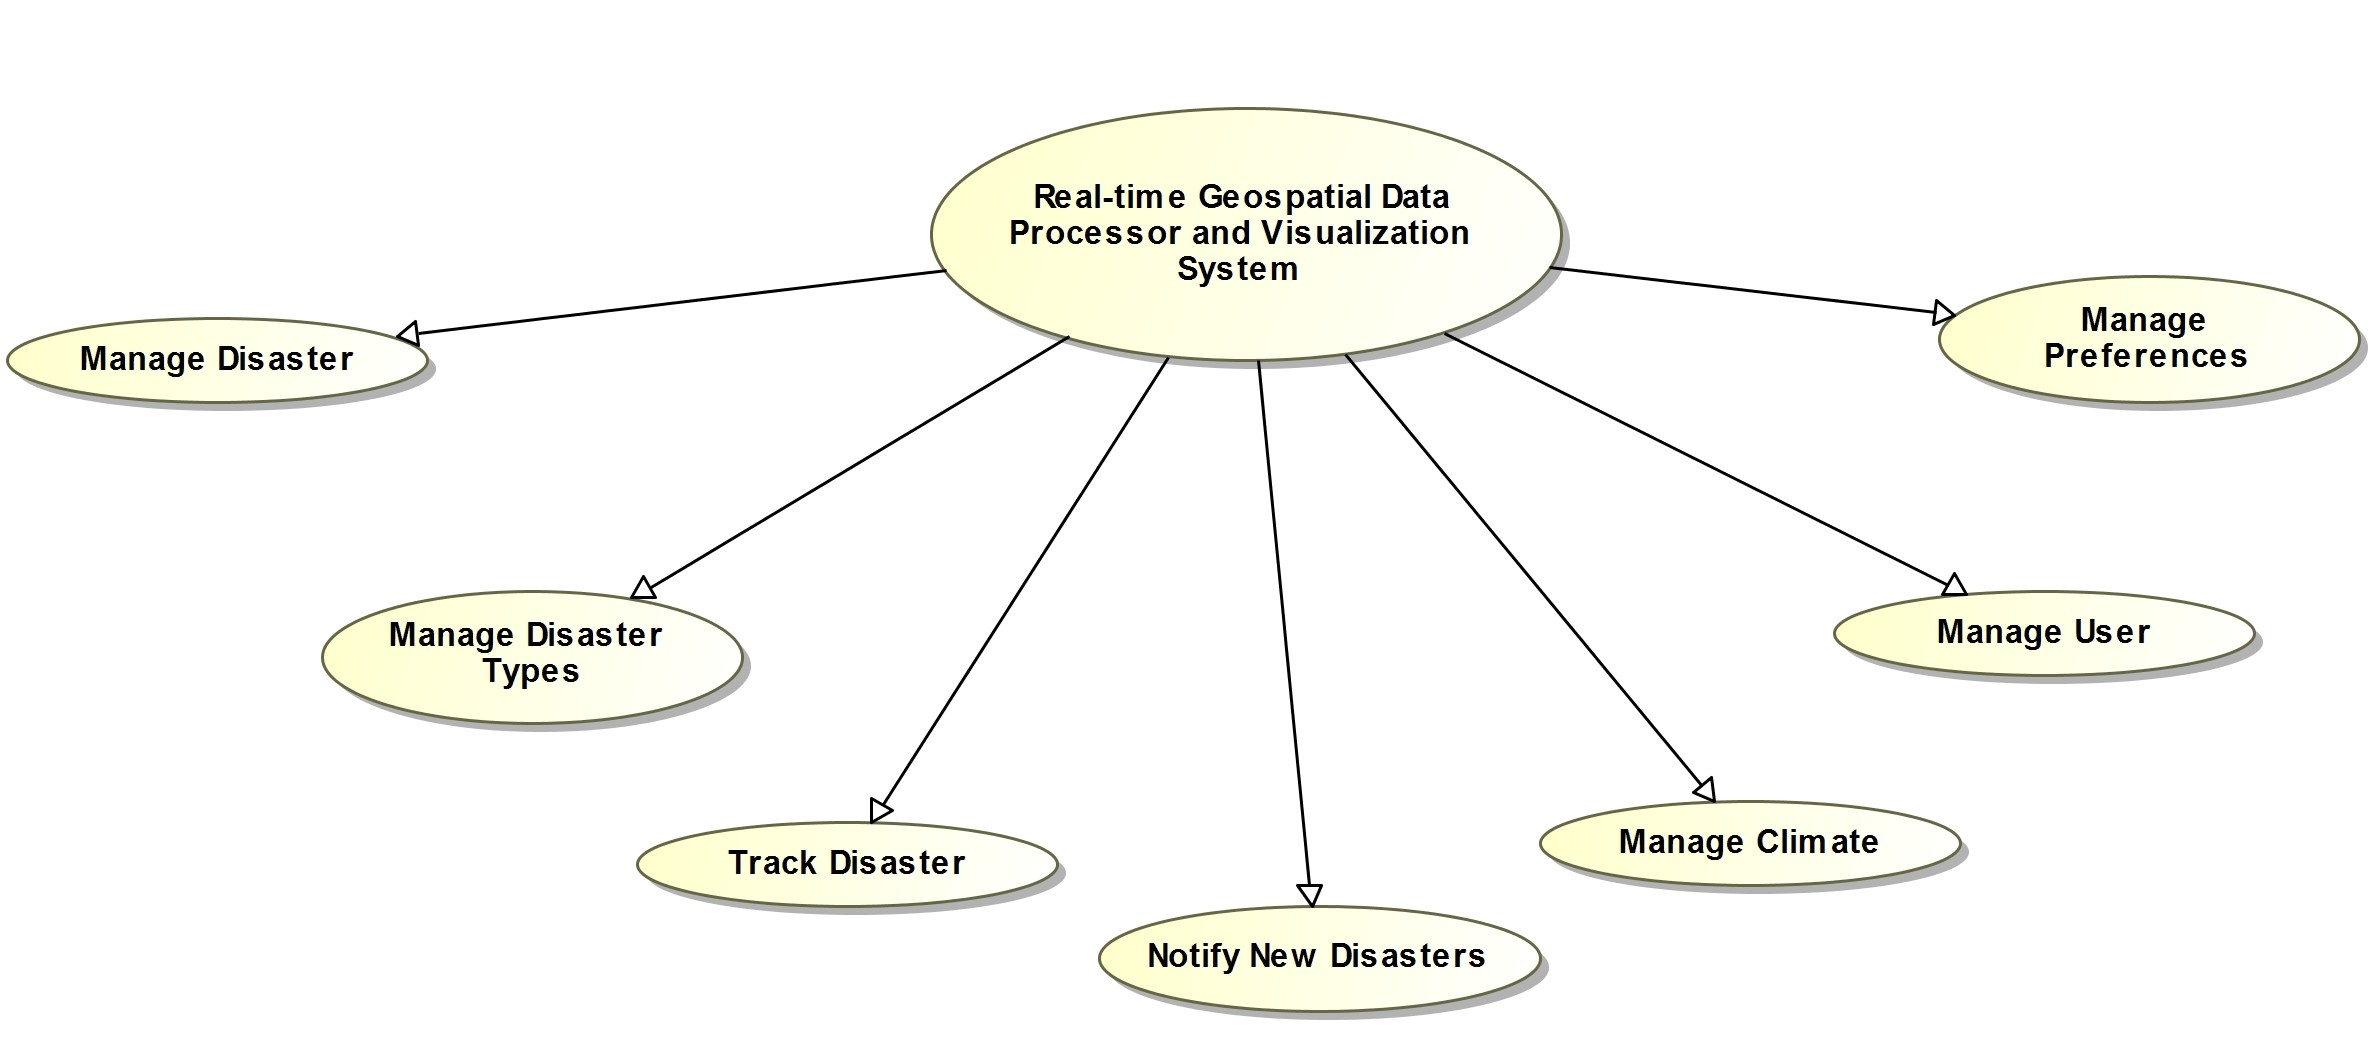
\includegraphics[width=90mm]{../images/funcReq/systOverview.jpg}
\caption{ Overview of the System \label{overflow}}
\end{figure}
		\subsection{Use Cases}
		Below is a list of all the use cases we have identified thus far:
\begin{itemize}%[listparindent=1.5em, labelsep=2em, itemindent=1.5em]
	\item \textbf{Manage Disaster}\\ Manage disaster is the use case that allows the user to query a specific disaster by type and time.
	\item \textbf{Track Disaster} \\ Track disaster use case allows the user to track an active disaster. they will be able to get any new updates on the currently active disasters.
	\item \textbf{Manage Disaster Types} \\ Manage Disaster Types allows an Admin user to add disaster types to the system.
	\item \textbf{Notify New Disaster} \\ Notify New Disaster notifies a currently online user if there are any disasters that have just became active. 
	\item \textbf{Manage Climate} \\ This use case is similar to the manage disaster use case except that the user can only view climate details.
	\item \textbf{Manage User} \\ This use case allows users to register their details to the system, as well as login and log out of the system.
	\item \textbf{Manage Preferences} \\ This use case allows a logged in user to add, edit or view their weather or disaster preferences.
\end{itemize}
		
		\subsection{Use Case Prioritization}
		The system use cases are characterised as follows:
 \begin{itemize}

 	\item \textbf{Manage Disaster - Critical}\\ This use case is critical since the main functionality of the system requires disaster management.
 	\item \textbf{Manage Disaster Types - Important}\\ An authorized user should be able to add a new disaster type or remove a redundant disaster type.
	\item \textbf{Track Disaster - Important}\\ Users need to be able to track an active disaster that has occurred for feedback purposes. 
 	\item \textbf{Notify New Disaster - Important}\\ A user that is currently online should be able to get instantaneous notification of a newly occurring disaster.
 	\item \textbf{Manage Climate - Important}\\ A user should be able to view normal weather climate at any time they wish to.
 	\item \textbf{Manage User - Important} \\ A user should be able to register with the system because as a registered user they are able to access all the functionality provided by the system.  An authorized user (admin) once logged in is able to access and/or modify relevant system data.
	\item \textbf{Manage Preferences - Important} \\ A registered user should be able to add, edit or view their weather and disaster preferences.
 \end{itemize}
		
	\section{Modular System}		
		\subsection{Disaster Management Module}
		\subsubsection{Scope}

\begin{figure}[H]
	\centering
	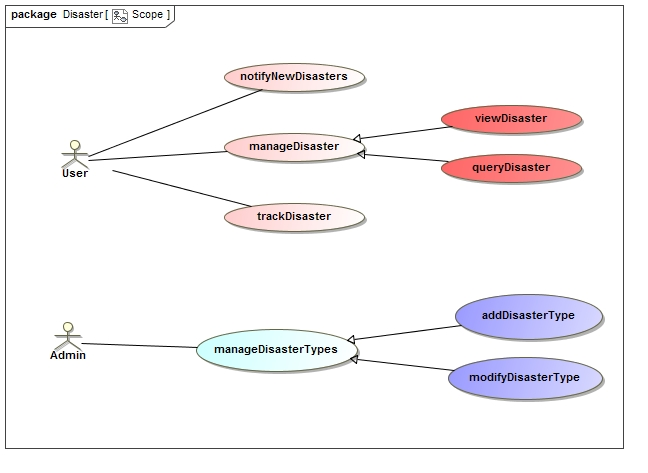
\includegraphics[scale=0.77]{../images/funcReq/DisasterScope.jpg}
	\caption{The scope of functionality required from the disaster module \label{overflow}}
\end{figure}

Admin can add and/or modify the different kinds of disaster types that are required whilst users are able to track and manage disasters as well as get notifications for new disasters. 

\subsubsection{viewDisaster}

A user can view disasters by going on to the disasters tab on the system and being able to view all the active disasters that are occurring throughout the world. Below are the service contract, activity diagram and functional requirements diagram for viewDisaster.

\begin{figure}[H]
	\centering
	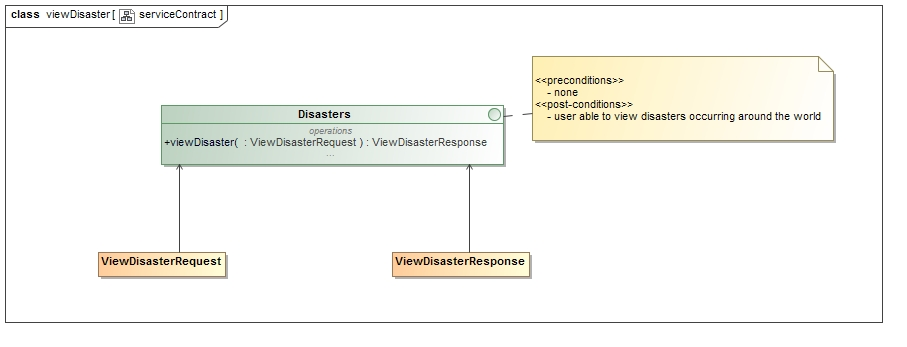
\includegraphics[width=1.0\textwidth]{../images/funcReq/viewDisasterServiceContract.jpg}
	\caption{The service contract for viewDisaster \label{overflow}}
\end{figure}

\begin{figure}[H]
	\centering
	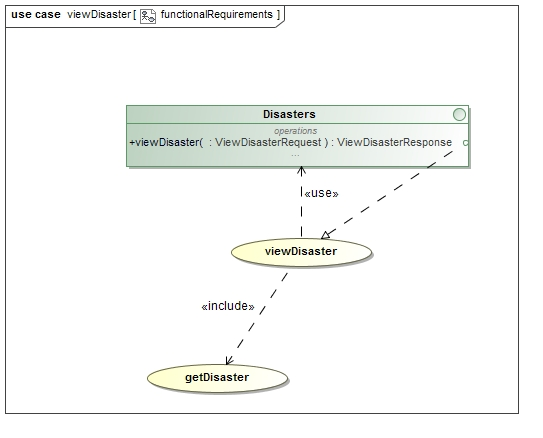
\includegraphics[width=1.0\textwidth]{../images/funcReq/viewDisasterFunctionalRequirements.jpg}
	\caption{The functional requirements diagram for viewDisaster \label{overflow}}
\end{figure}

\begin{figure}[H]
	\centering
	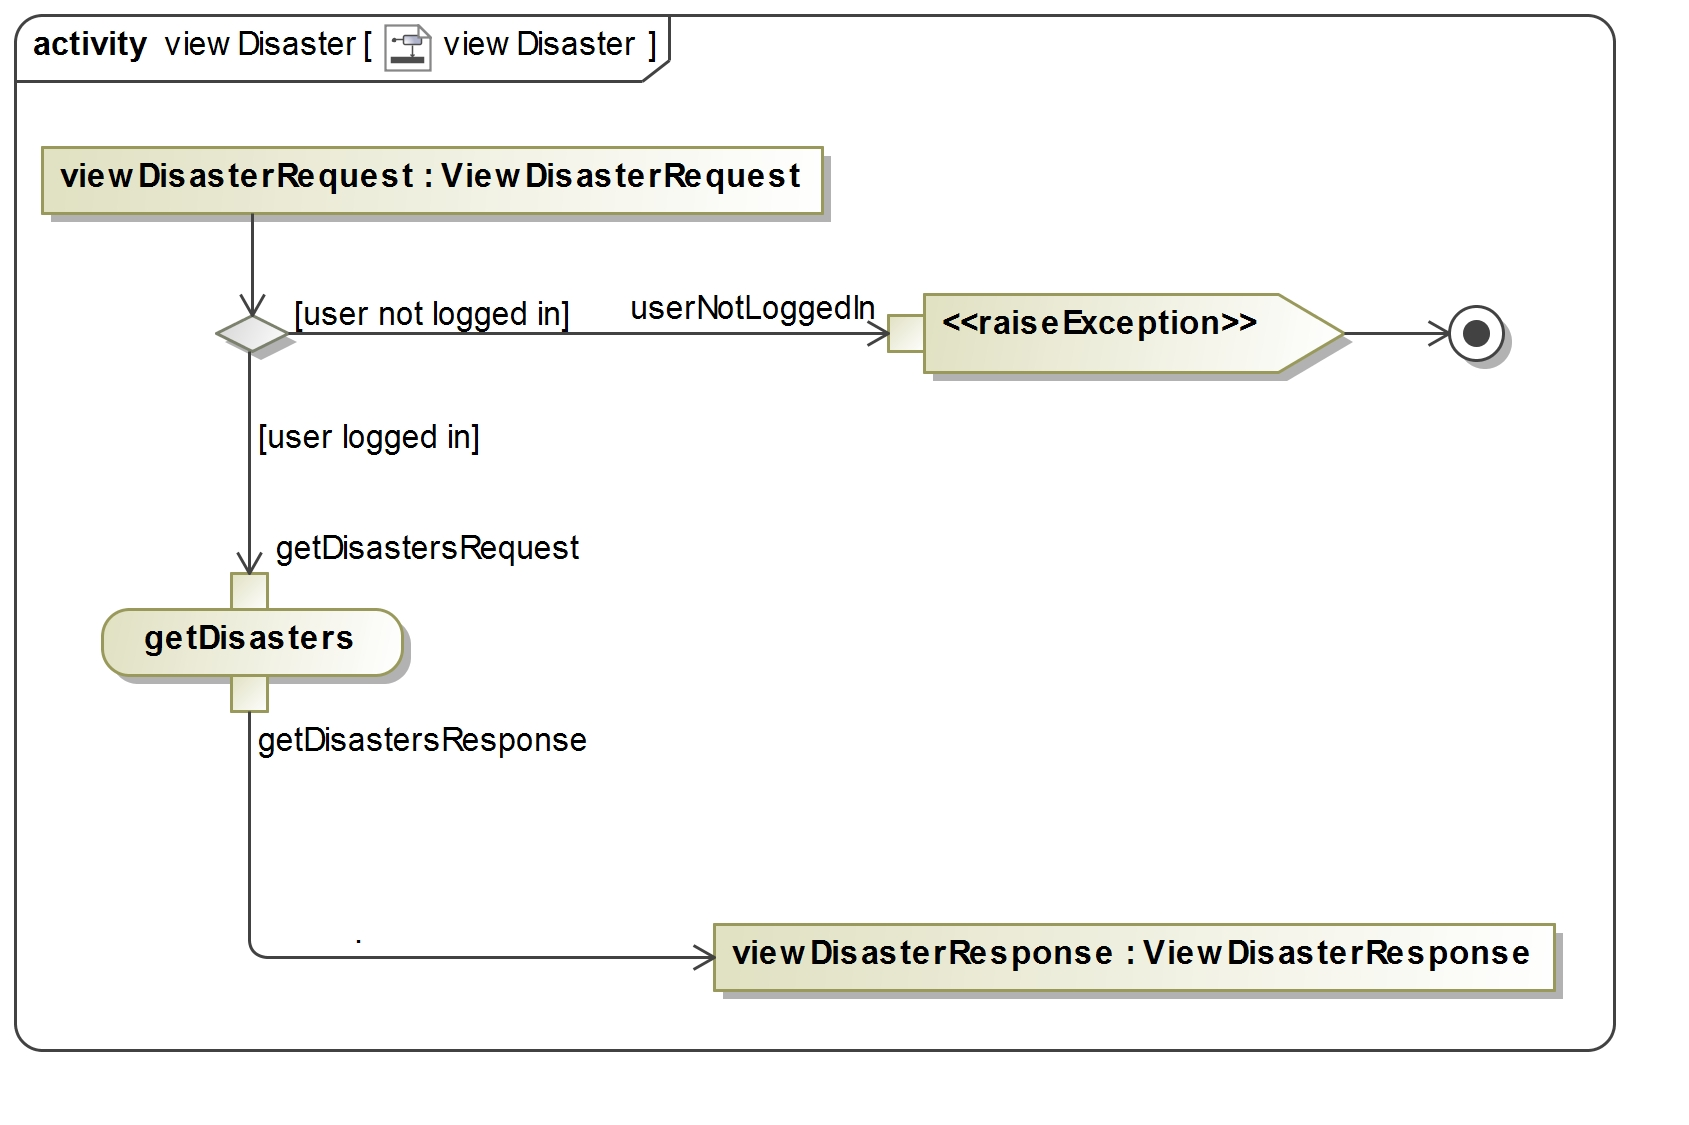
\includegraphics[width=1.0\textwidth]{../images/funcReq/viewDisasterActivityDiagram.jpg}
	\caption{The activity diagram for viewDisaster \label{overflow}}
\end{figure}

\subsubsection{queryDisaster}

The user will be able to query the system for specific disasters, by entering search criteria, such as a start date and/or a end date, so that only disasters matching the specified criteria are returned to the user. Below are the service contract, activity diagram and functional requirements diagram for queryDisaster.

 \begin{figure}[H]
	\centering
	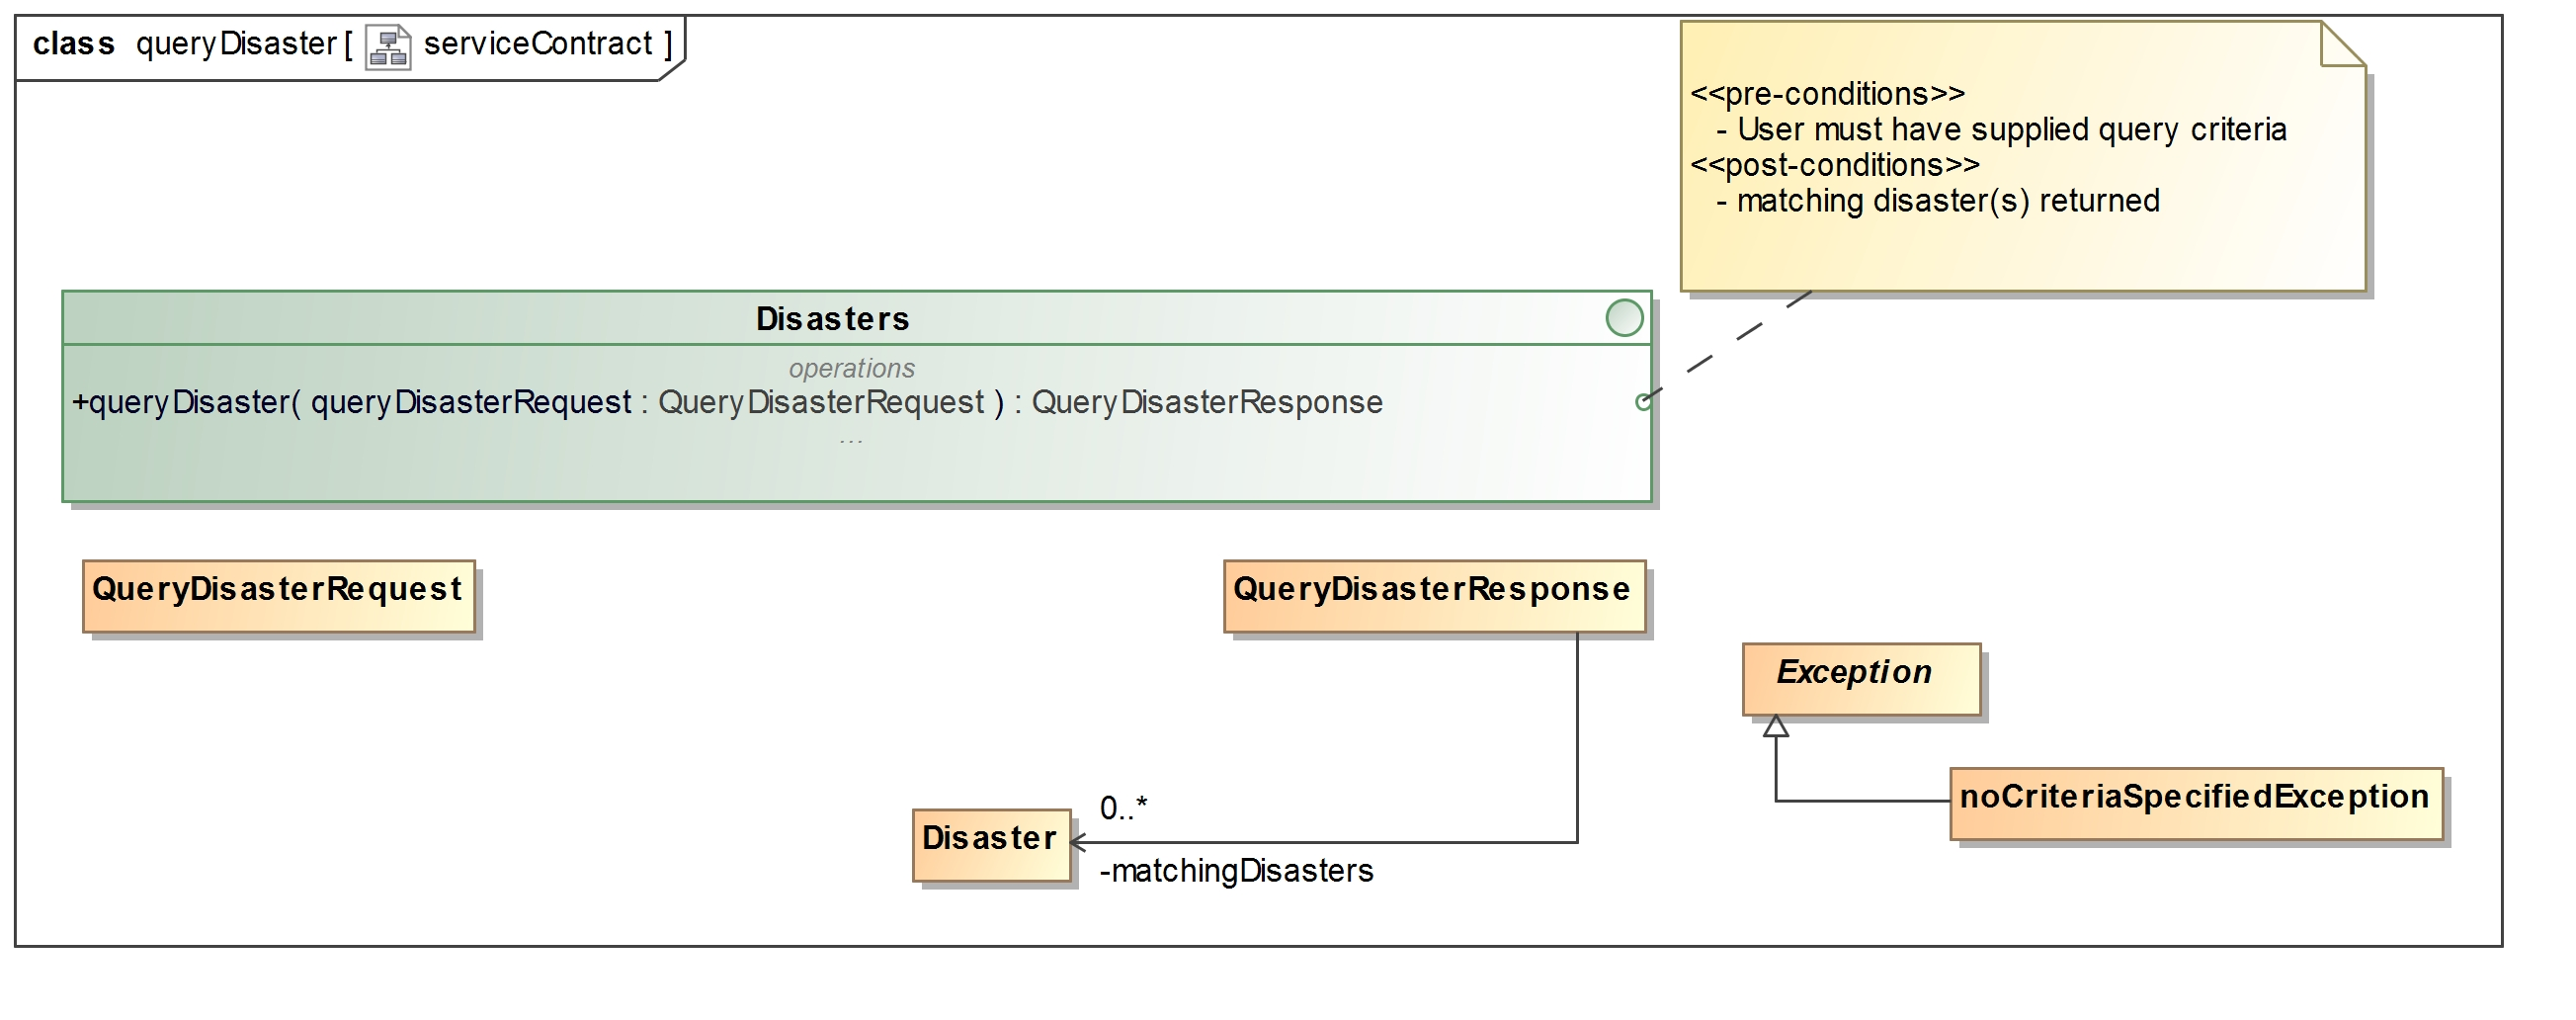
\includegraphics[width=1.0\textwidth]{../images/funcReq/queryDisasterServiceContract.jpg}
	\caption{The service contract for queryDisaster \label{overflow}}
\end{figure}

\begin{figure}[H]
	\centering
	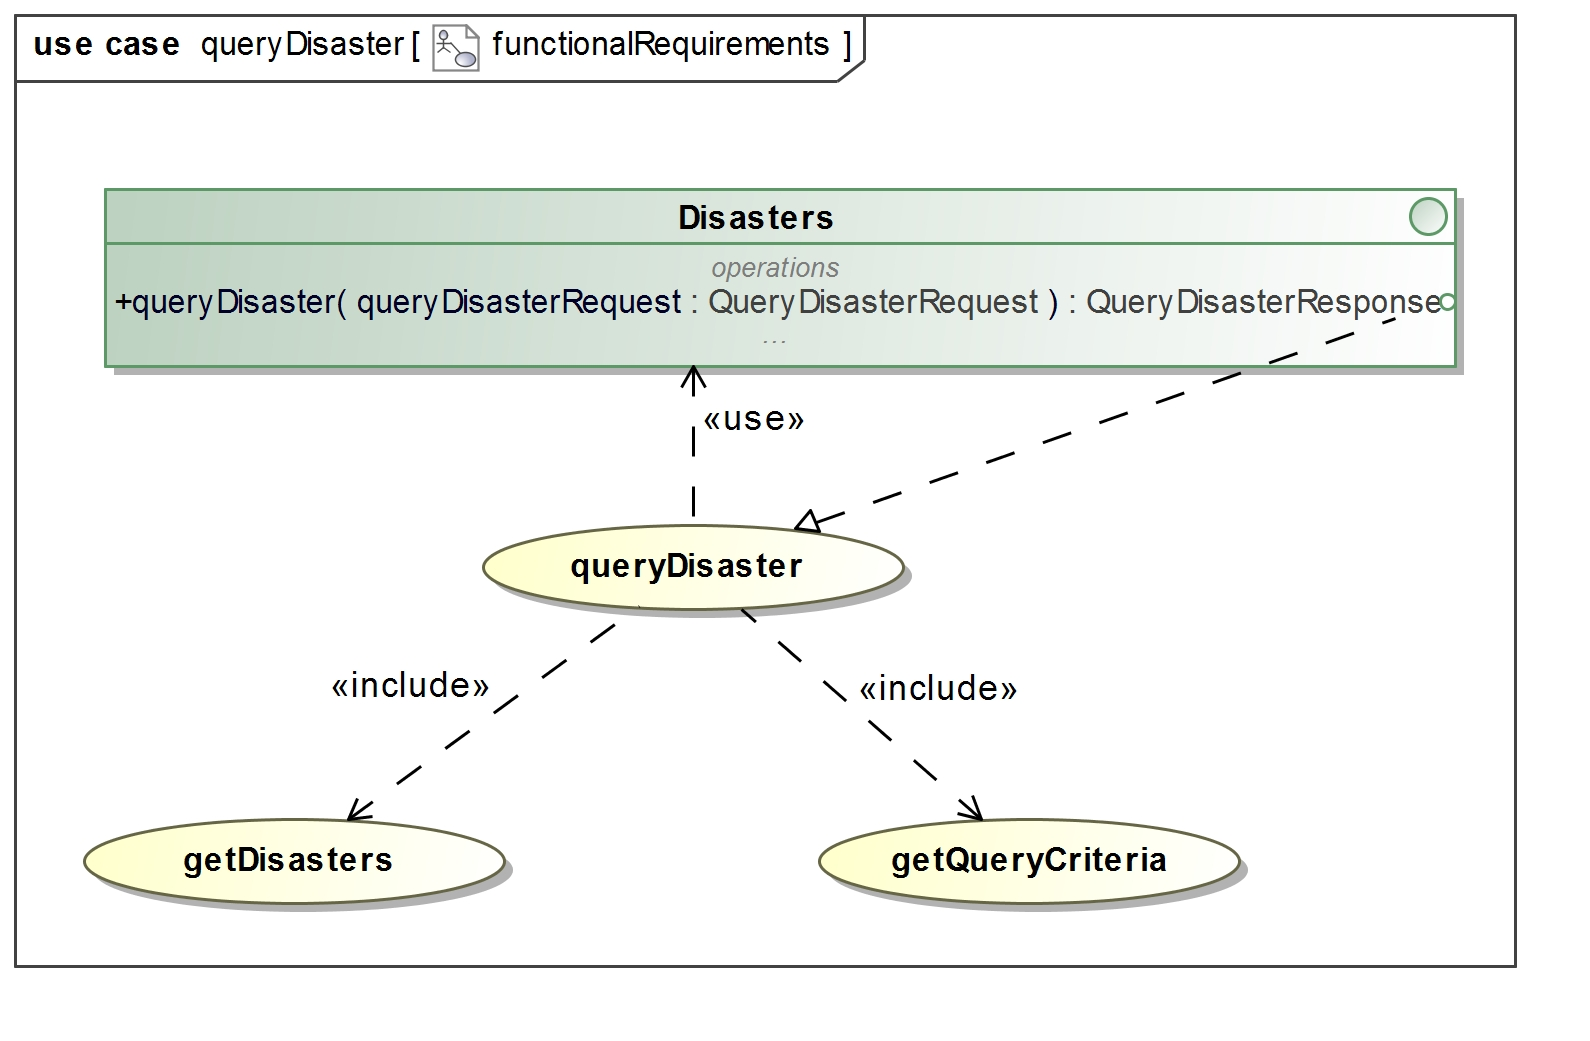
\includegraphics[width=1.0\textwidth]{../images/funcReq/queryDisasterFunctionalRequirements.jpg}
	\caption{The functional requirements diagram for queryDisaster \label{overflow}}
\end{figure}

\begin{figure}[H]
	\centering
	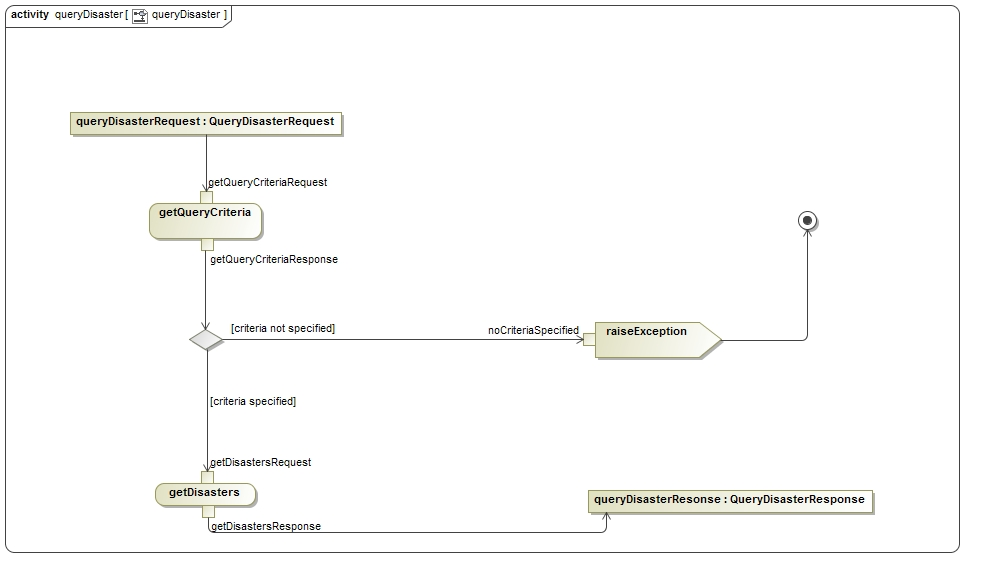
\includegraphics[width=1.0\textwidth]{../images/funcReq/queryDisasterActivityDiagram.jpg}
	\caption{The activity diagram for queryDisaster \label{overflow}}
\end{figure} 

\subsubsection{notifyNewDisaster}

A user will be able to be notified of any new disasters that are occuring as of the time they are using the system. Below are the service contract, activity diagram and functional requirements diagram for notifyNewDisaster.

 \begin{figure}[H]
	\centering
	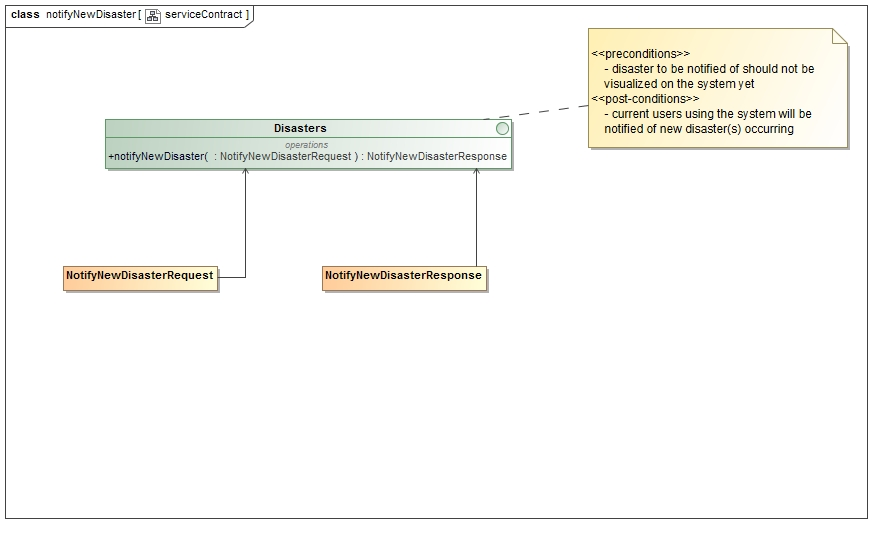
\includegraphics[width=1.0\textwidth]{../images/funcReq/notifyNewDisasterServiceContract.jpg}
	\caption{The service contract for notifyNewDisaster \label{overflow}}
\end{figure}

\begin{figure}[H]
	\centering
	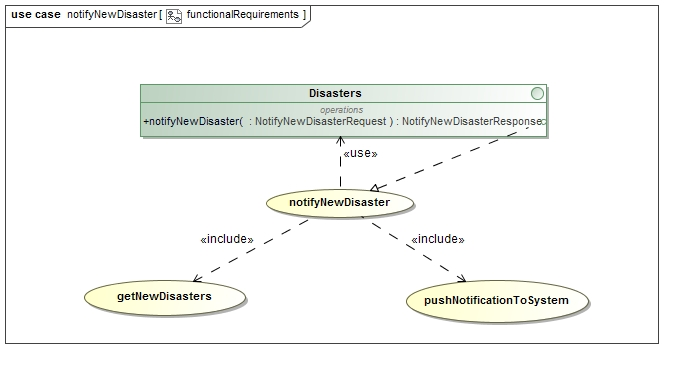
\includegraphics[width=1.0\textwidth]{../images/funcReq/notifyNewDisasterFunctionalRequirements.jpg}
	\caption{The functional requirements diagram for notifyNewDisaster \label{overflow}}
\end{figure}

\begin{figure}[H]
	\centering
	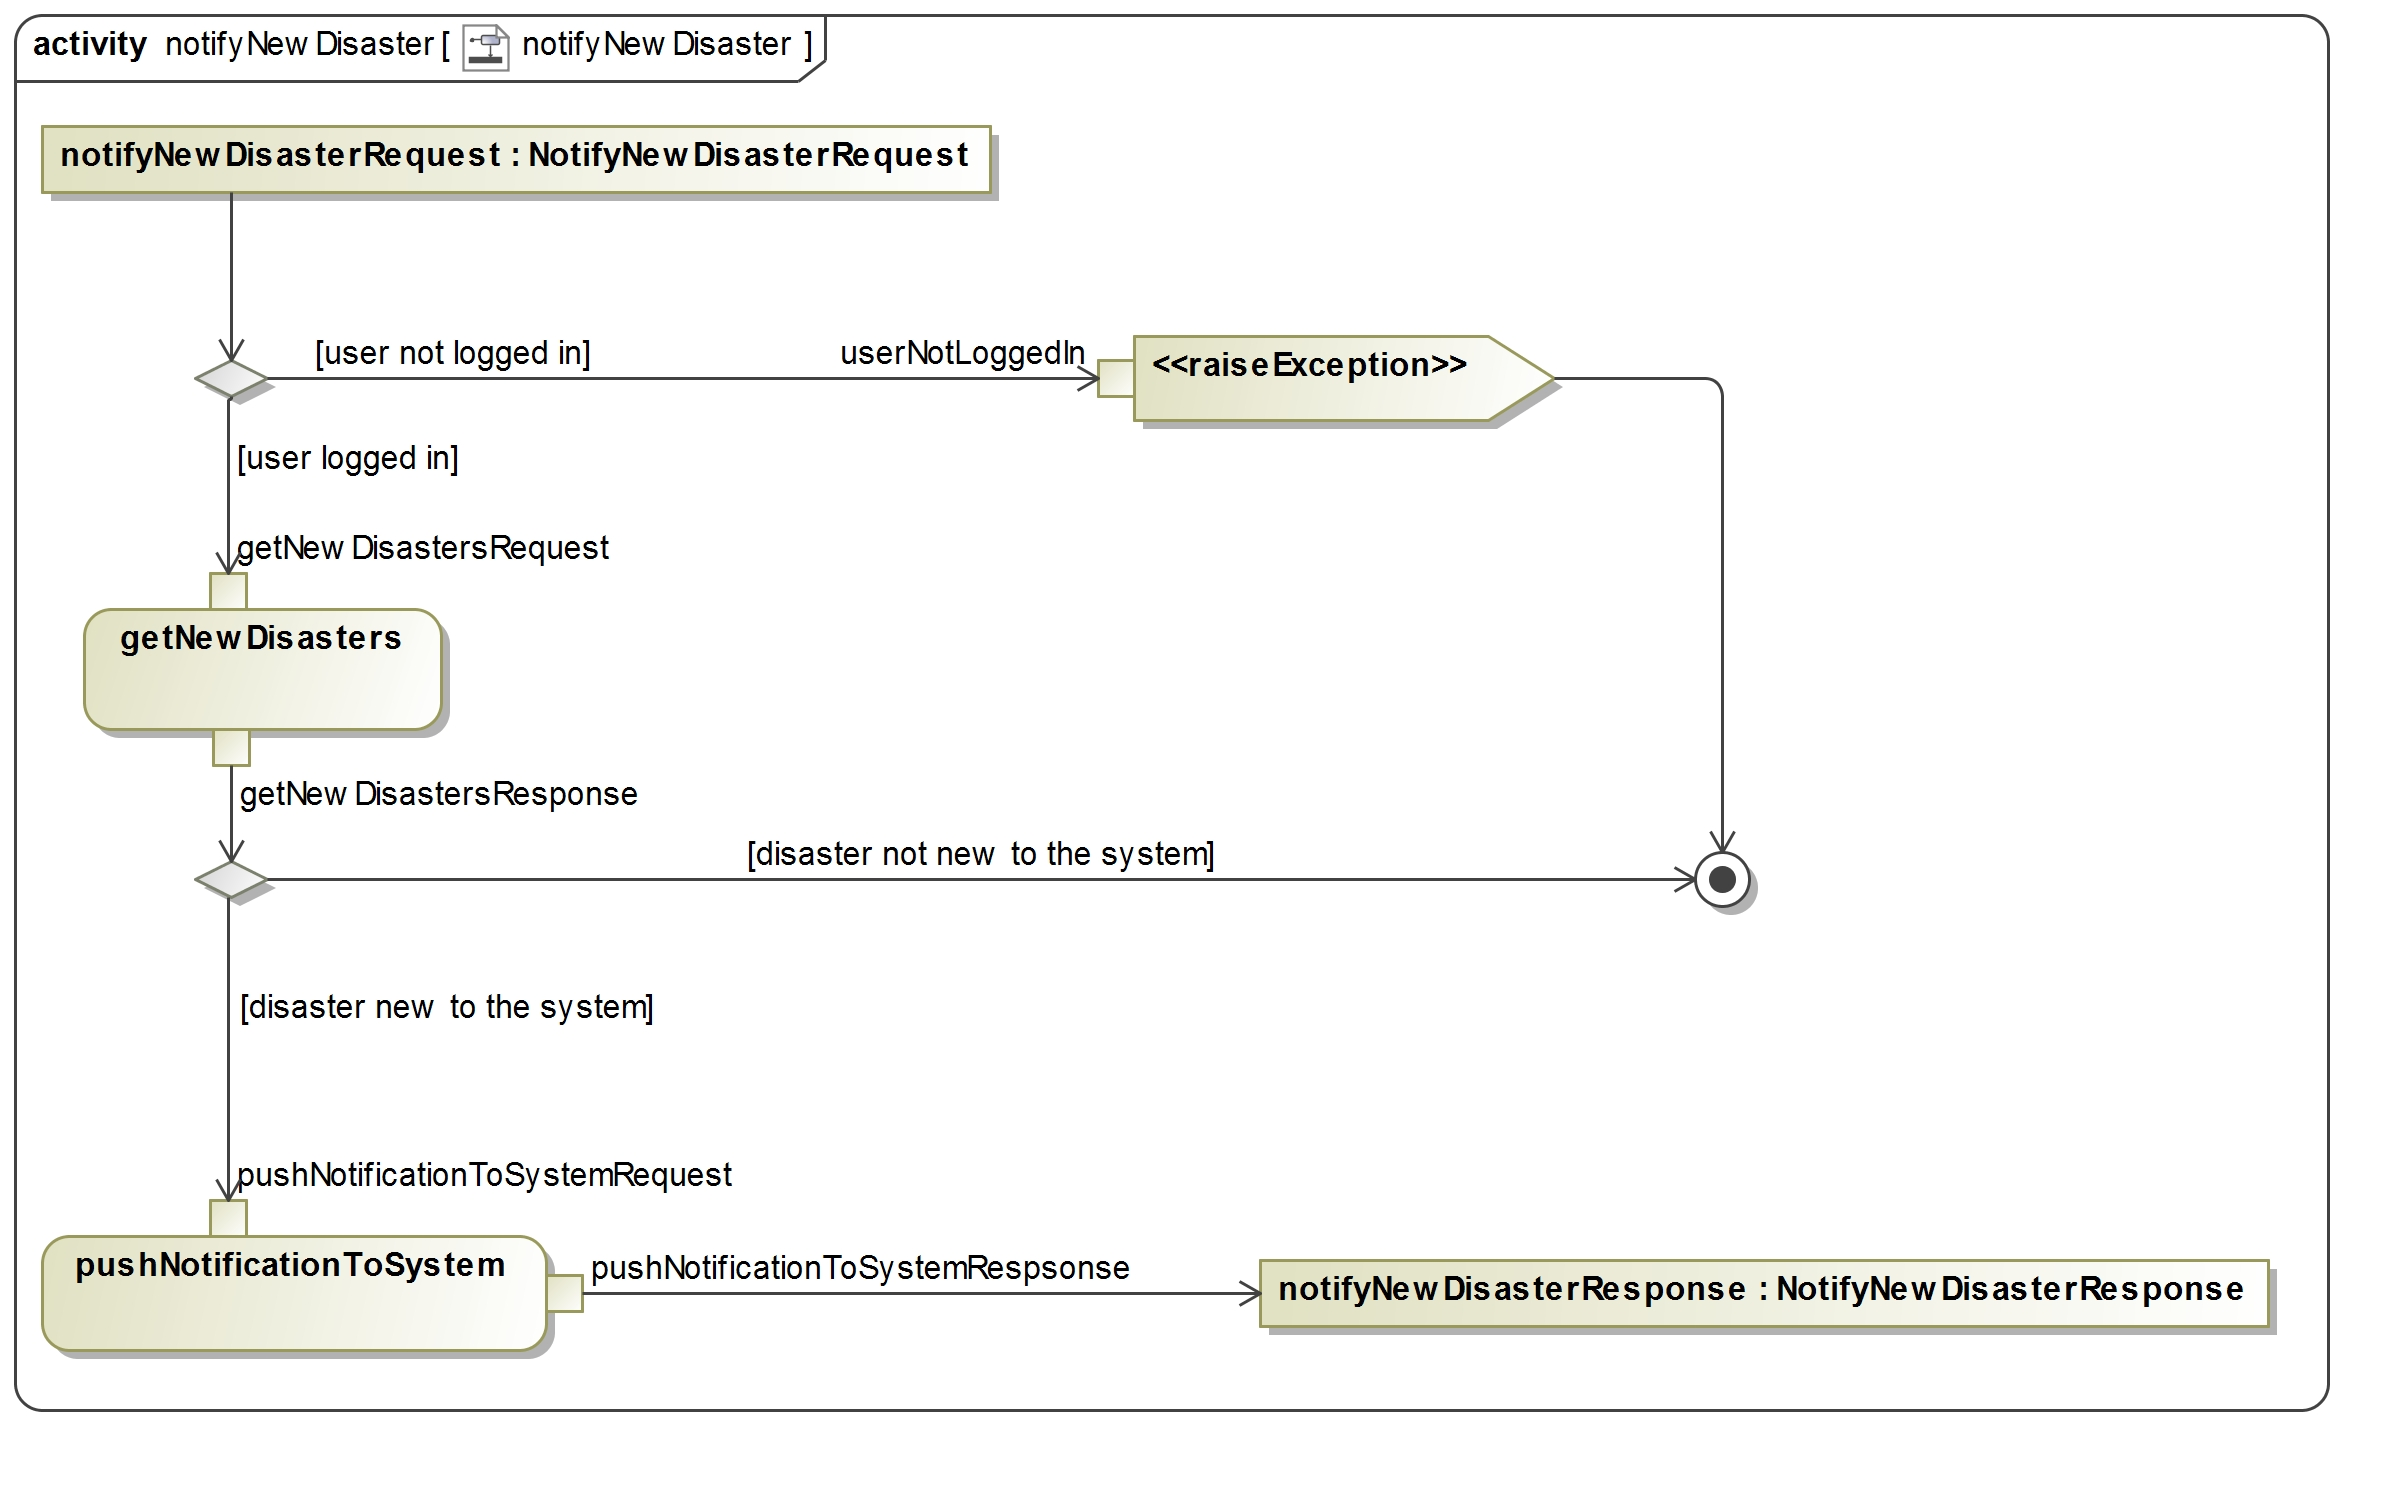
\includegraphics[width=1.0\textwidth]{../images/funcReq/notifyNewDisasterActivityDiagram.jpg}
	\caption{The activity diagram for notifyNewDisaster \label{overflow}}
\end{figure} 

\subsubsection{addDisasterType}

Adding a disaster type requires that the user has admin rights and that there should not be a disaster type of the same name as the one being added that exists. If the user is admin and the disaster type being added is unique then a new disaster type will be added to the system. Below are the service contract, activity diagram and functional requirements diagram for addDisasterType.

\begin{figure}[H]
	\centering
	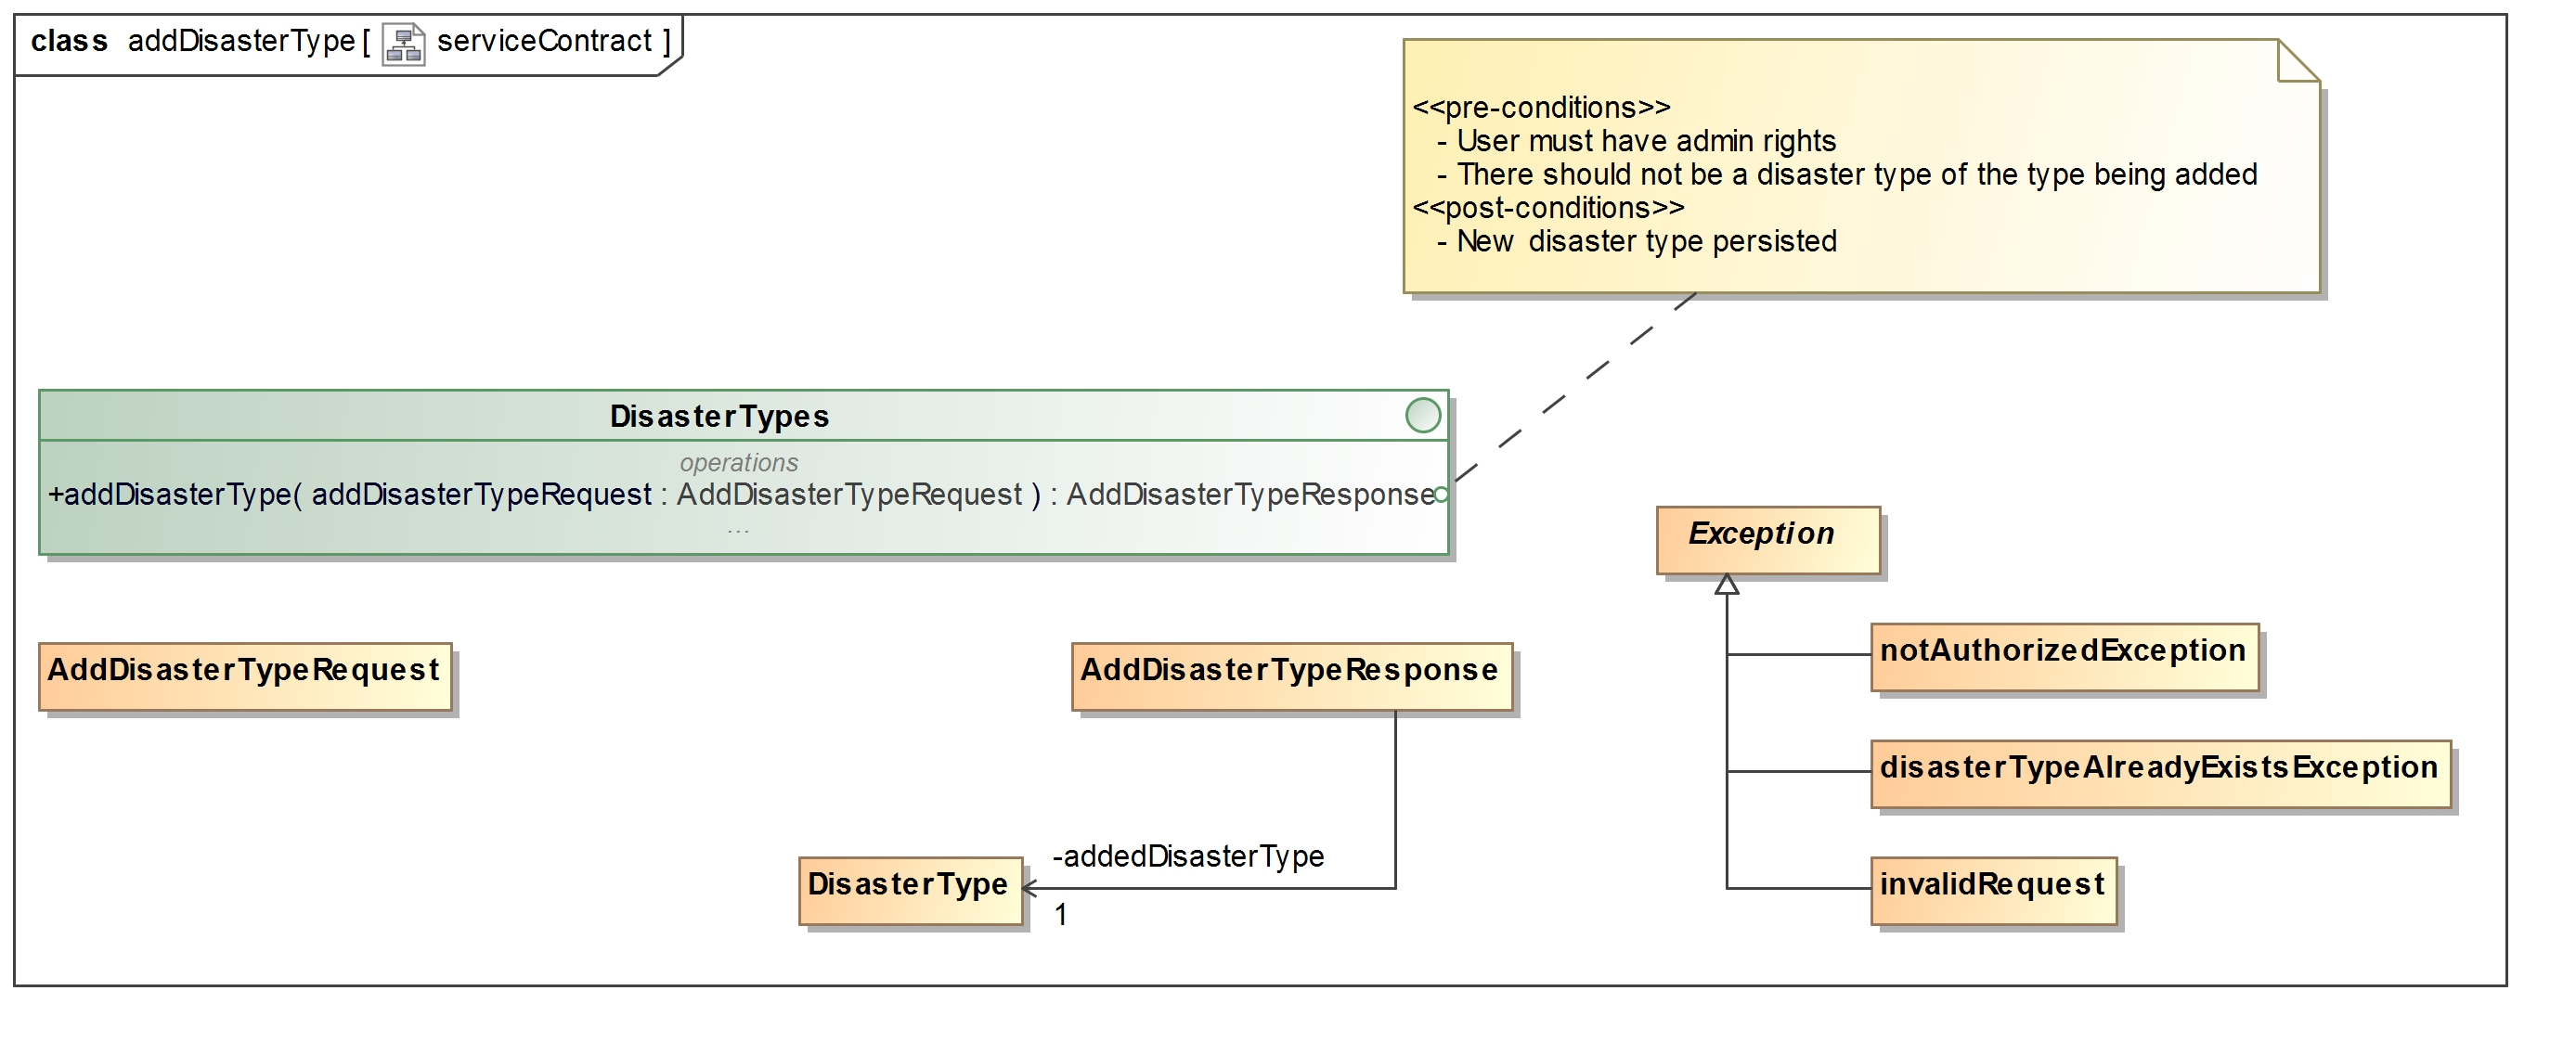
\includegraphics[width=1.0\textwidth]{../images/funcReq/addDisasterTypeServiceContract.jpg}
	\caption{The service contract for addDisasterType \label{overflow}}
\end{figure}

\begin{figure}[H]
	\centering
	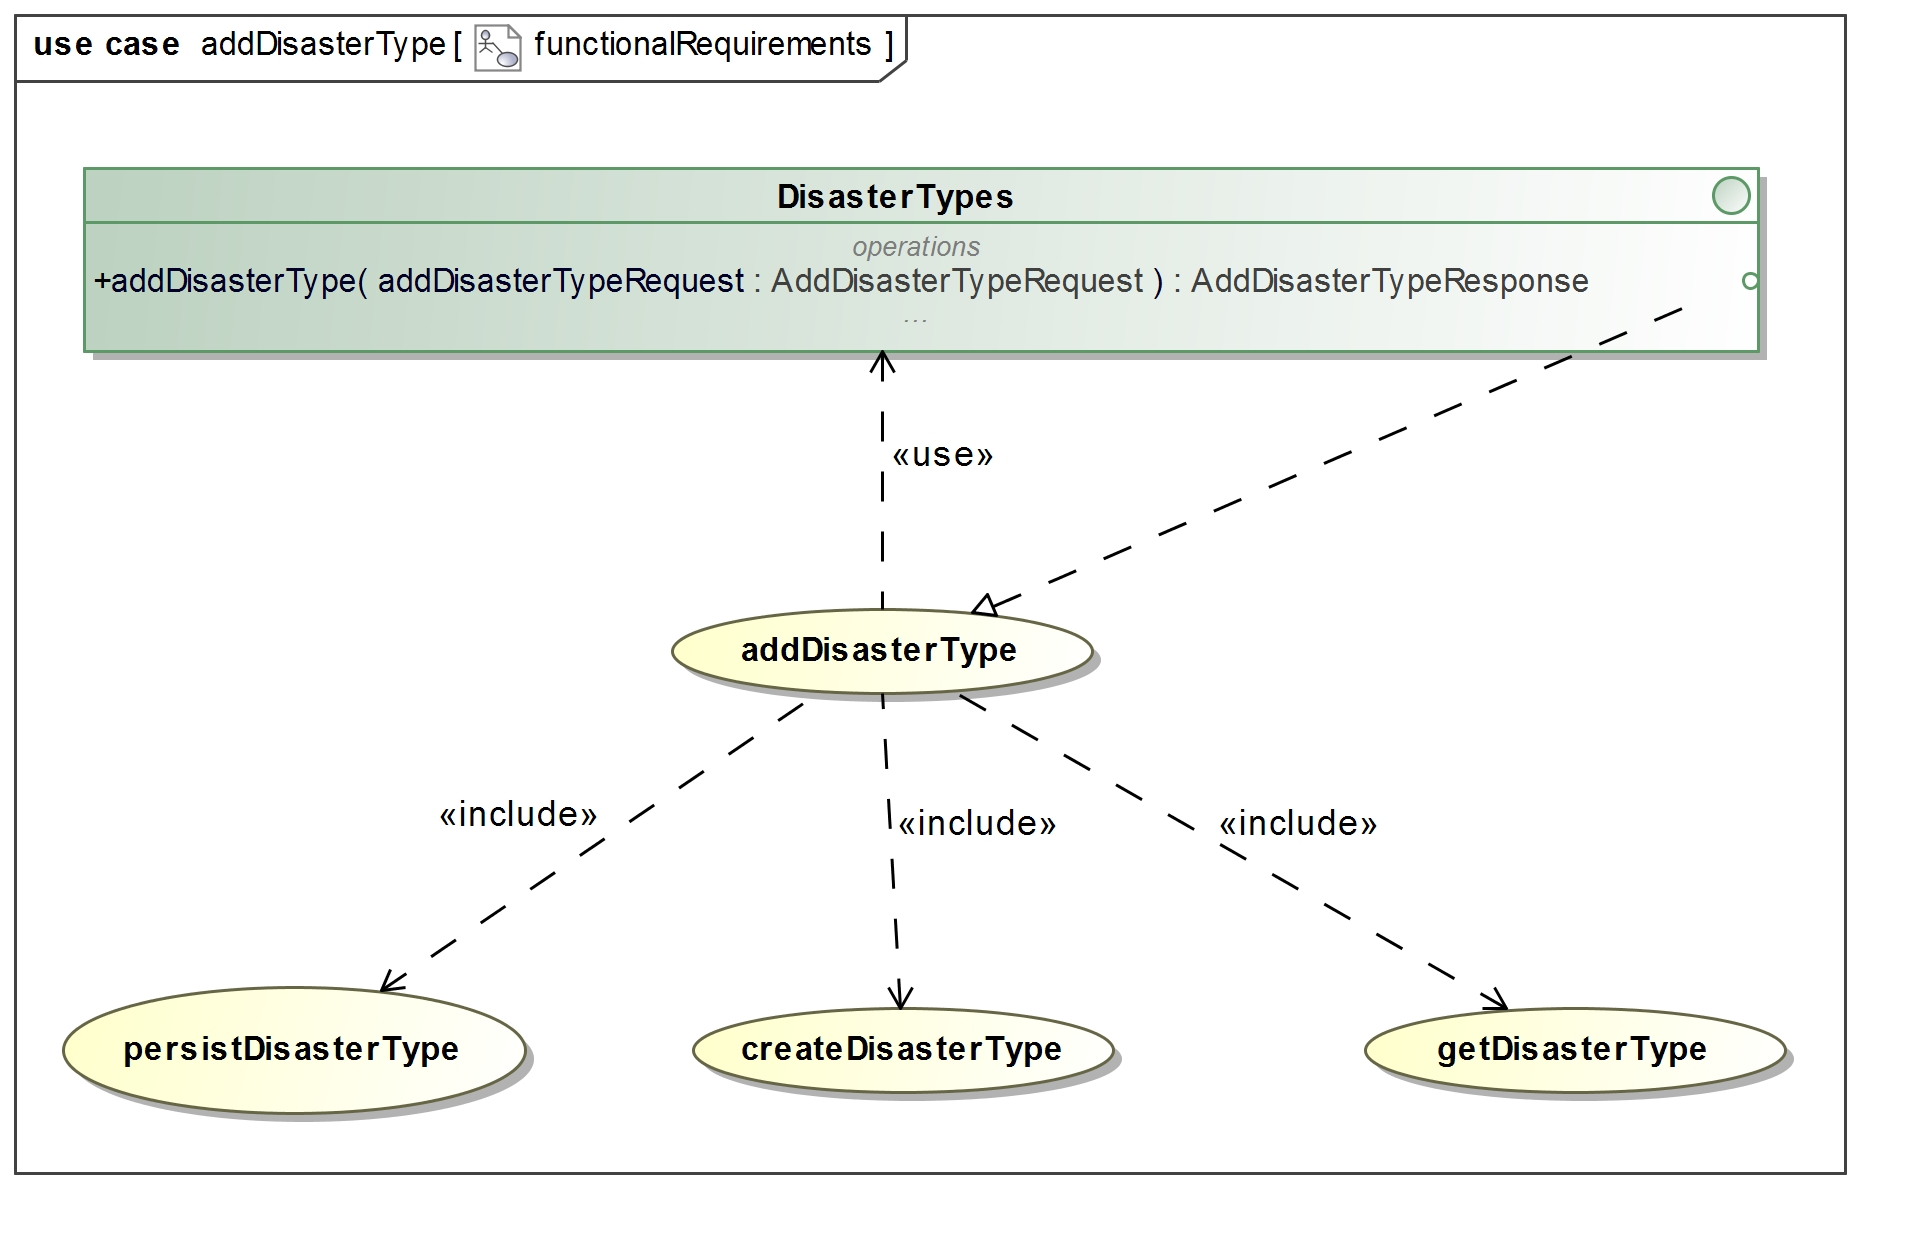
\includegraphics[width=1.0\textwidth]{../images/funcReq/AddDisasterTypeFunctionalRequirements.jpg}
	\caption{The functional requirements diagram for addDisasterType \label{overflow}}
\end{figure}

\begin{figure}[H]
	\centering
	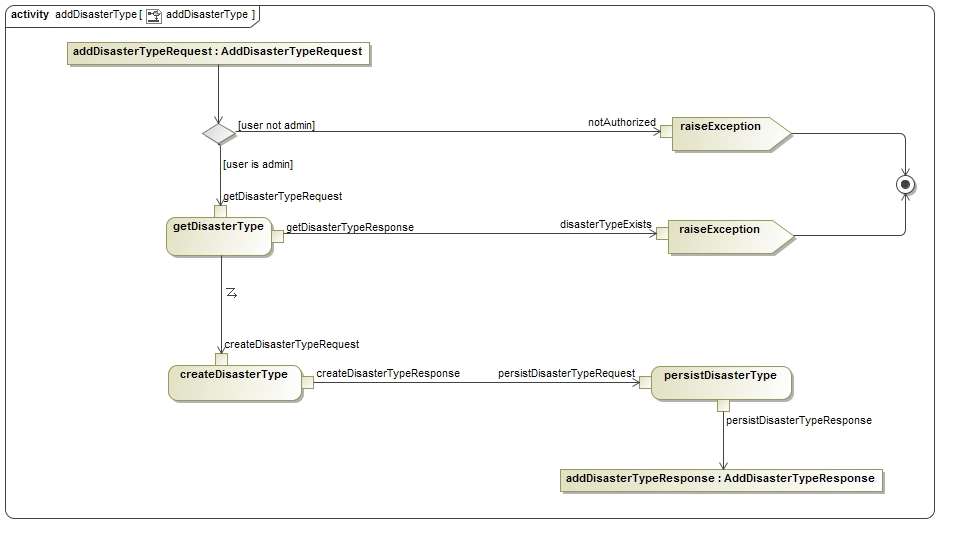
\includegraphics[width=1.0\textwidth]{../images/funcReq/addDisasterTypeActivityDiagram.jpg}
	\caption{The activity diagram for addDisasterType \label{overflow}}
\end{figure}

\subsubsection{modifyDisasterType}

Modifying a disaster type requires that the user has admin rights and that there should not be a disaster type of the same name as the modified one that exists. If the user is admin and the modified disaster type is unique then the modified disaster type will be persisted to the database. Below are the service contract, activity diagram and functional requirements diagram for modifiyDisasterType.

\begin{figure}[H]
	\centering
	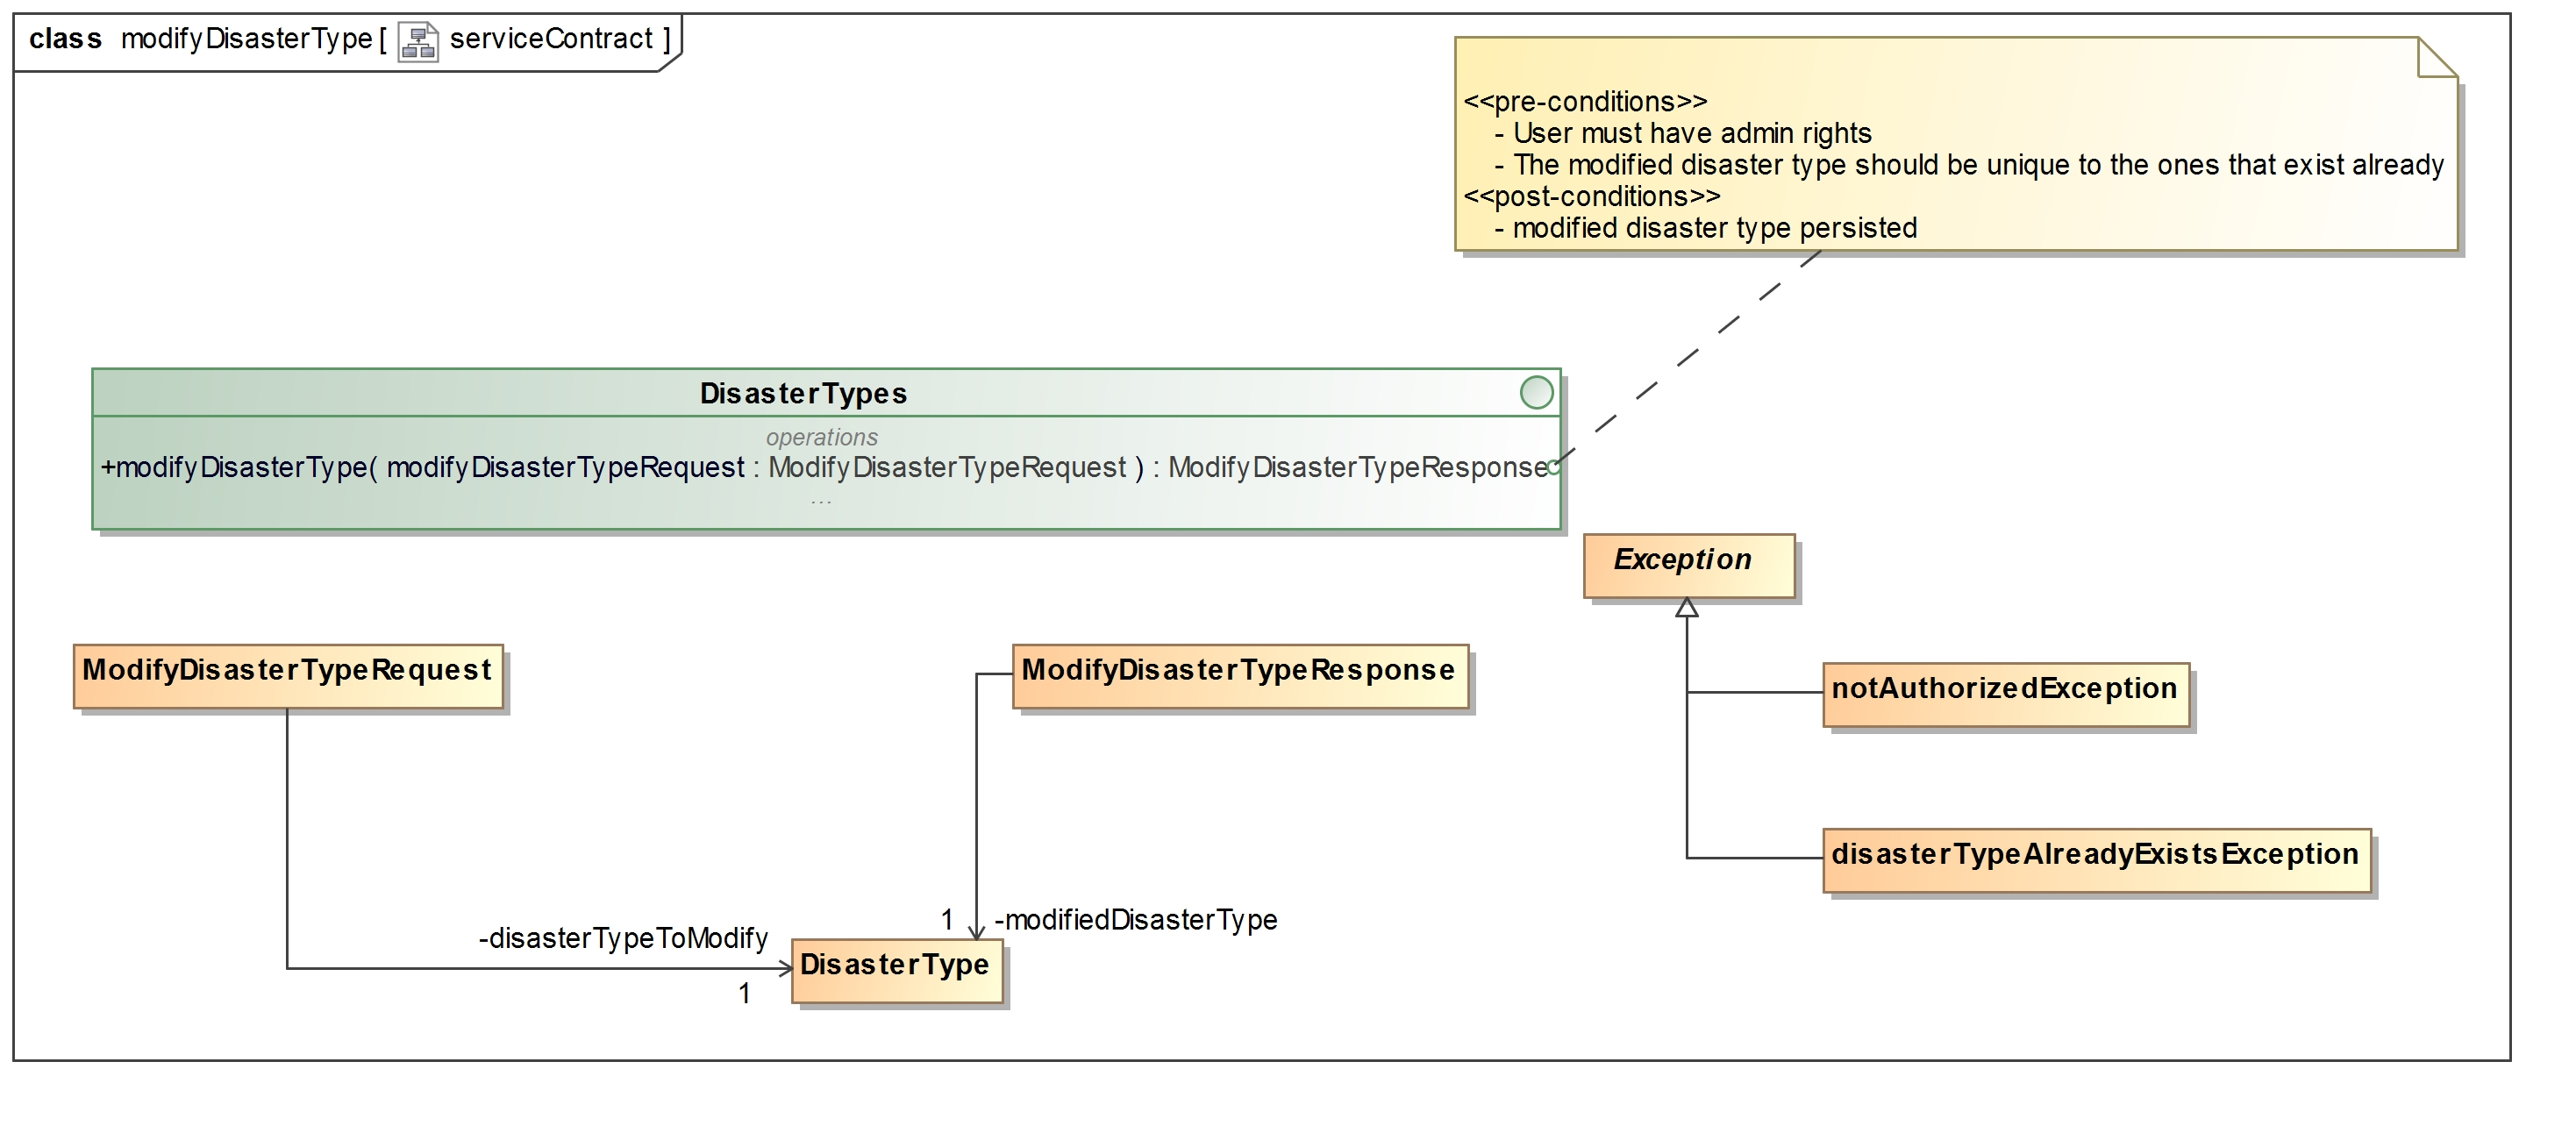
\includegraphics[width=1.0\textwidth]{../images/funcReq/modifyDisasterTypeServiceContract.jpg}
	\caption{The service contract for modifyDisasterType \label{overflow}}
\end{figure}

\begin{figure}[H]
	\centering
	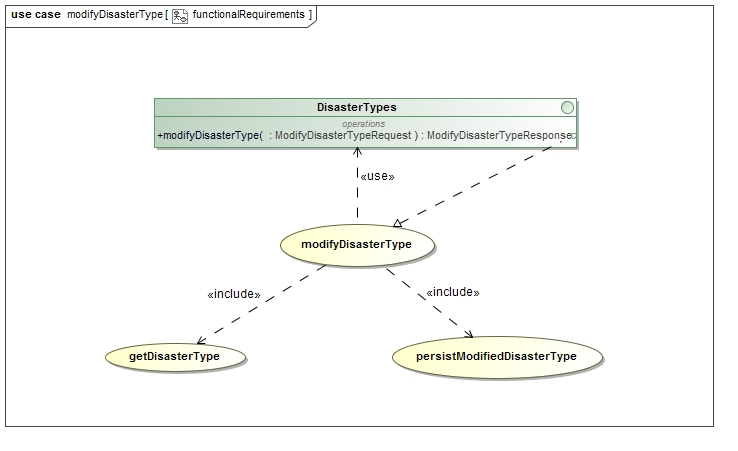
\includegraphics[width=1.0\textwidth]{../images/funcReq/modifyDisasterTypeFunctionalRequirements.jpg}
	\caption{The functional requirements diagram for modifyDisasterType \label{overflow}}
\end{figure}

\begin{figure}[H]
	\centering
	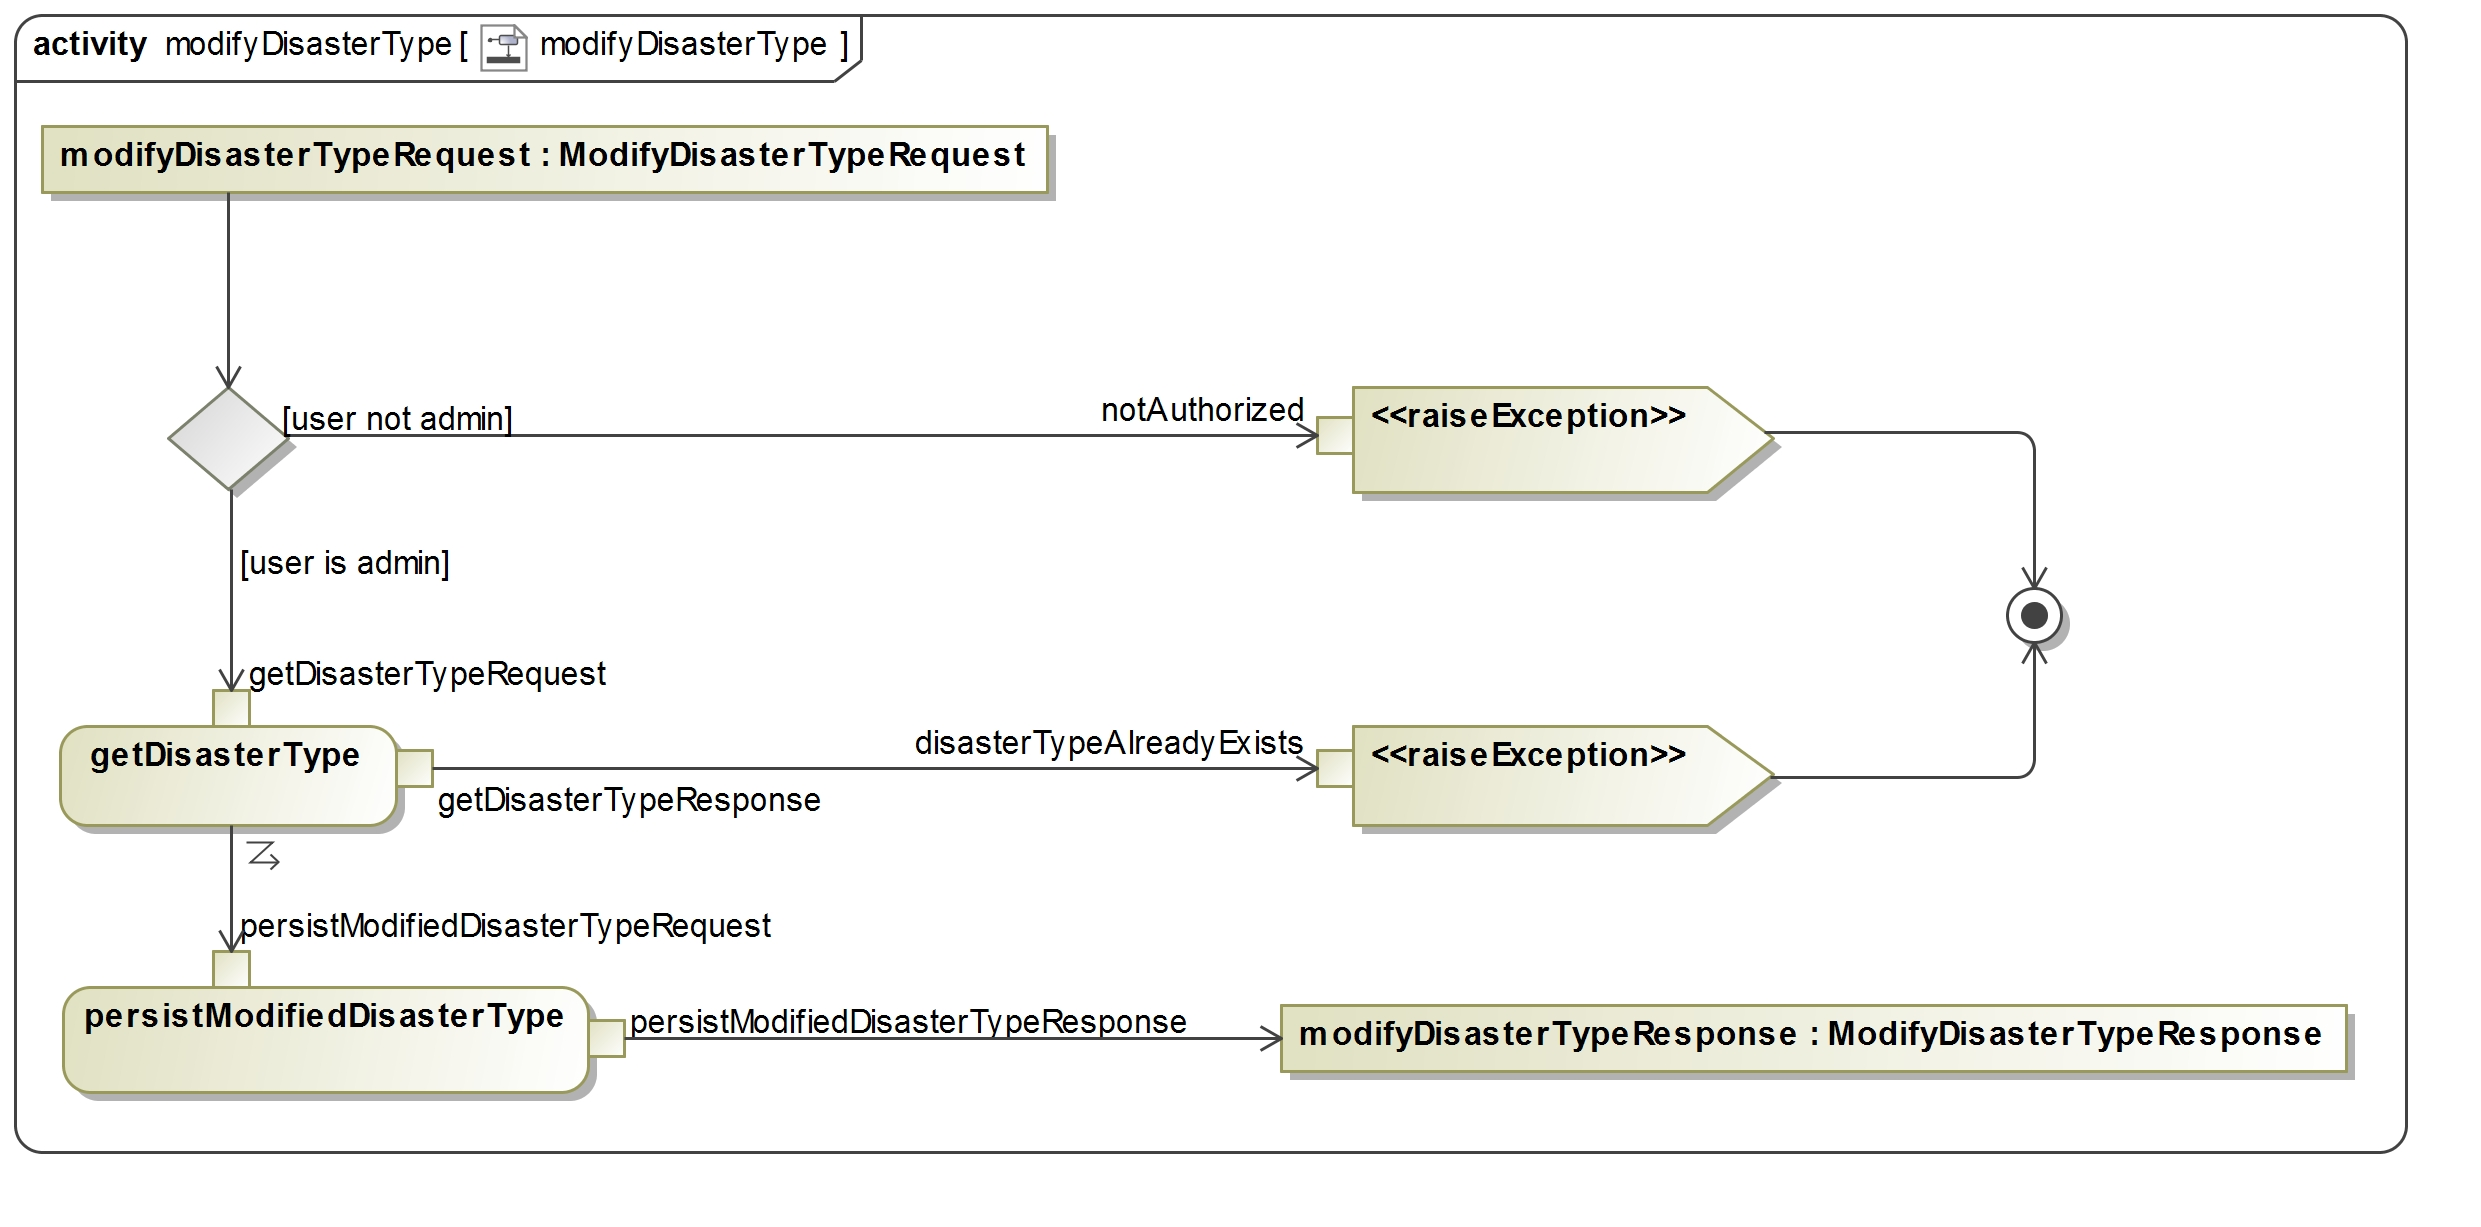
\includegraphics[width=1.0\textwidth]{../images/funcReq/modifyDisasterTypeActivityDiagram.jpg}
	\caption{The activity diagram for modifyDisasterType \label{overflow}}
\end{figure}

\subsubsection{trackDisaster}

	

	
		\subsection{Climate Management Module}
		\subsubsection{Scope}

\begin{figure}[H]
	\centering
	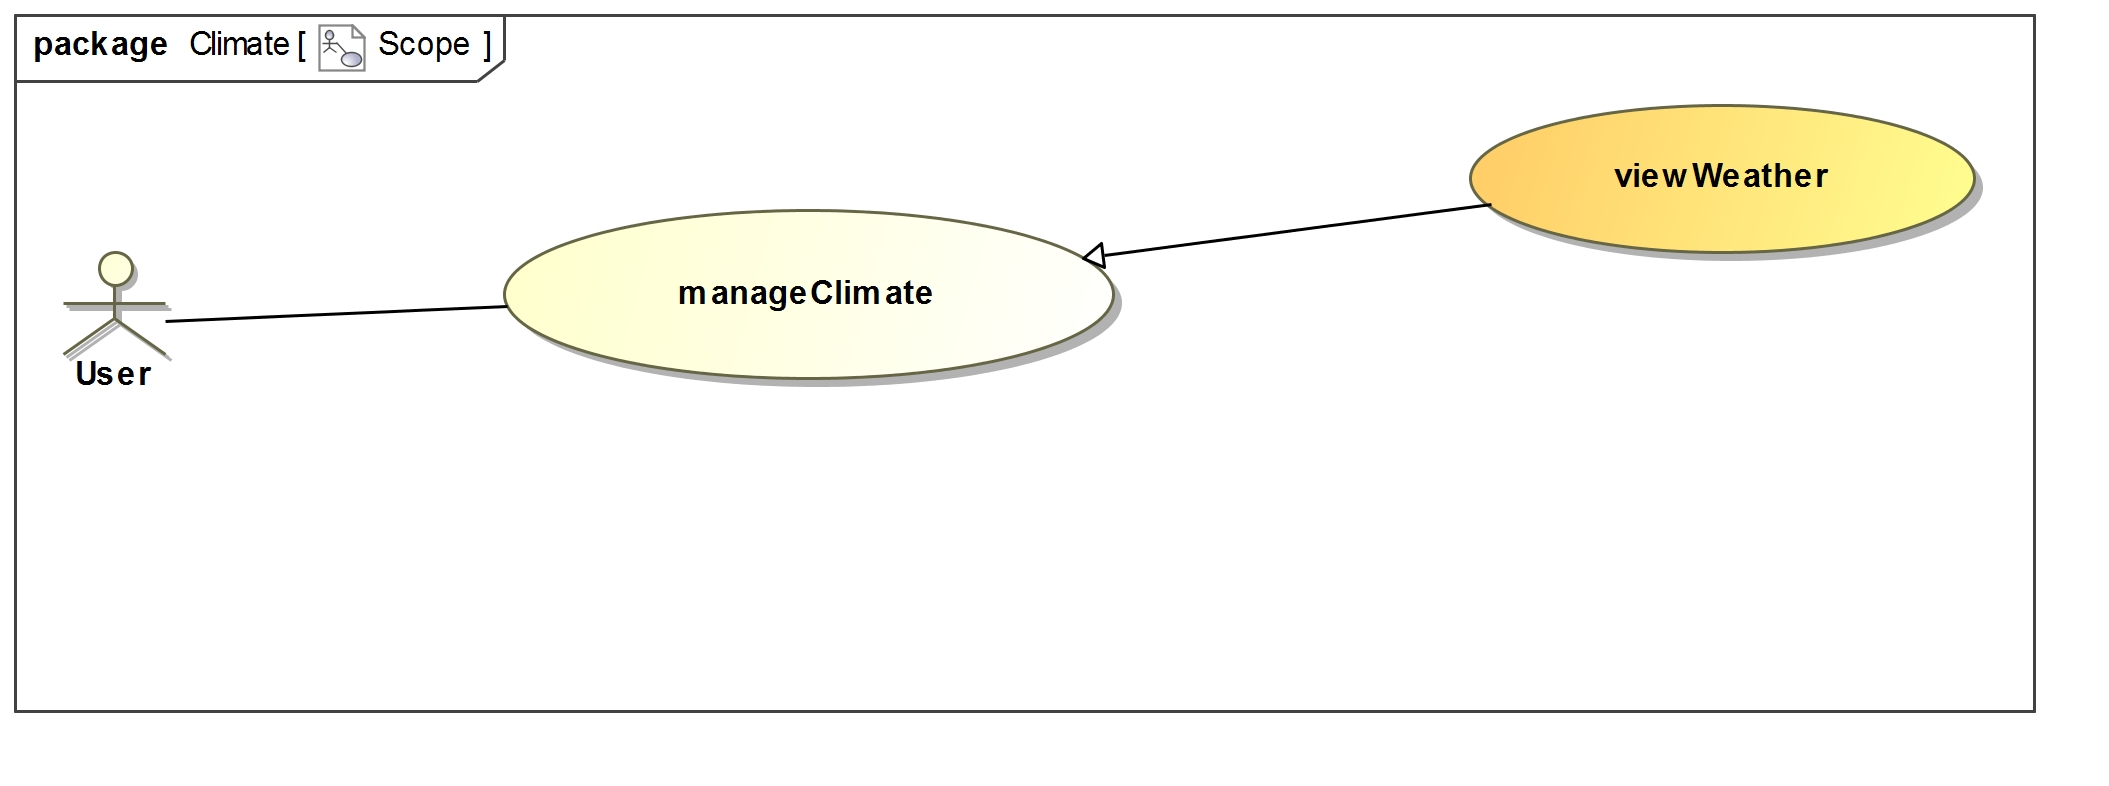
\includegraphics[scale=0.3]{../images/funcReq/ClimateScope.jpg}
	\caption{The scope of functionality required from the climate module \label{overflow}}
\end{figure} Users are able to view weather and query forecasts.

\subsubsection{viewWeather}

A user can view weather immediately as they go into the system or by going on to the weather tab on the system. The user is able to see weather for the entire world or for a specific place by specifying that place in a search bar. Below are the service contract, activity diagram and functional requirements diagram for viewWeather.

\begin{figure}[H]
	\centering
	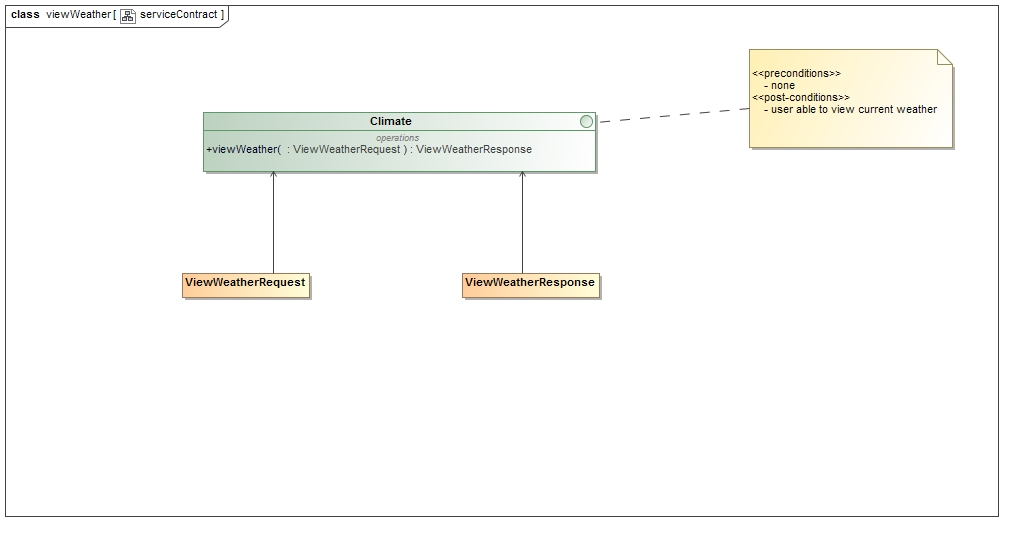
\includegraphics[width=1.0\textwidth]{../images/funcReq/viewWeatherServiceContract.jpg}
	\caption{The service contract for viewWeather \label{overflow}}
\end{figure}

\begin{figure}[H]
	\centering
	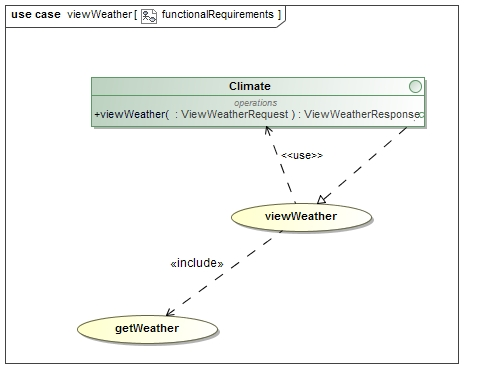
\includegraphics[width=1.0\textwidth]{../images/funcReq/viewWeatherFunctionalRequirements.jpg}
	\caption{The functional requirements diagram for viewWeather \label{overflow}}
\end{figure}

\begin{figure}[H]
	\centering
	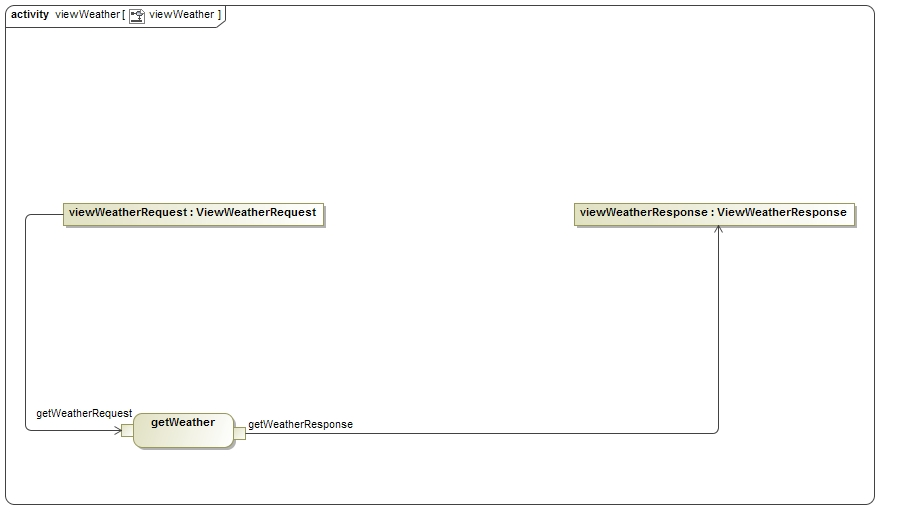
\includegraphics[width=1.0\textwidth]{../images/funcReq/viewWeatherActivityDiagram.jpg}
	\caption{The activity diagram for viewWeather \label{overflow}}
\end{figure}

\subsubsection{queryForecast}

A user is able to view the weather of a specific location for the next 5 days, given that they provide the latitude and longitude of that location.  Below are the service contract, activity diagram and functional requirements diagram for queryForecast.

\begin{figure}[H]
	\centering
	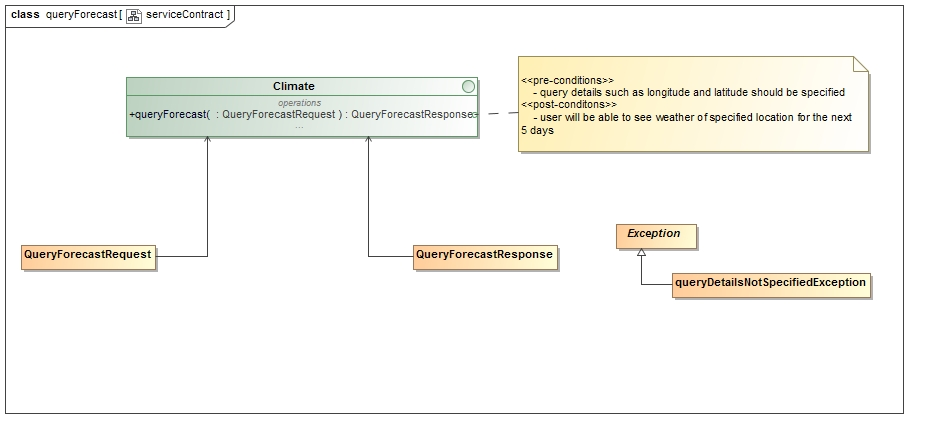
\includegraphics[width=1.0\textwidth]{../images/funcReq/queryForecastServiceContract.jpg}
	\caption{The service contract for queryForecast \label{overflow}}
\end{figure}

\begin{figure}[H]
	\centering
	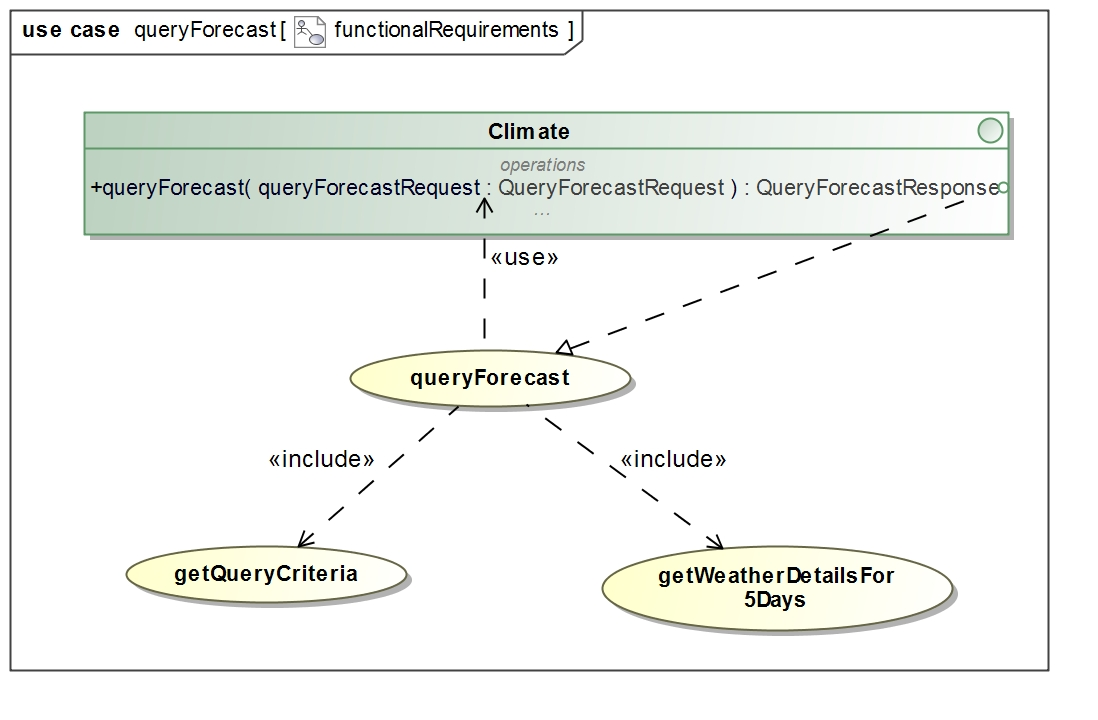
\includegraphics[width=1.0\textwidth]{../images/funcReq/queryForecastFunctionalRequirements.jpg}
	\caption{The functional requirements diagram for queryForecast \label{overflow}}
\end{figure}

\begin{figure}[H]
	\centering
	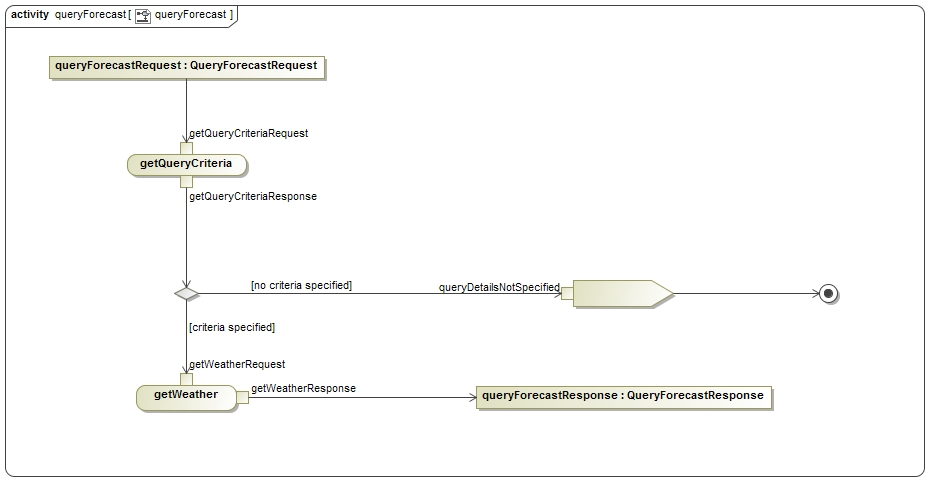
\includegraphics[width=1.0\textwidth]{../images/funcReq/queryForecastActivityDiagram.jpg}
	\caption{The activity diagram for queryForecast \label{overflow}}
\end{figure}	
		
		\subsection{User Module}
		\subsubsection{Scope}

\begin{figure}[H]
	\centering
	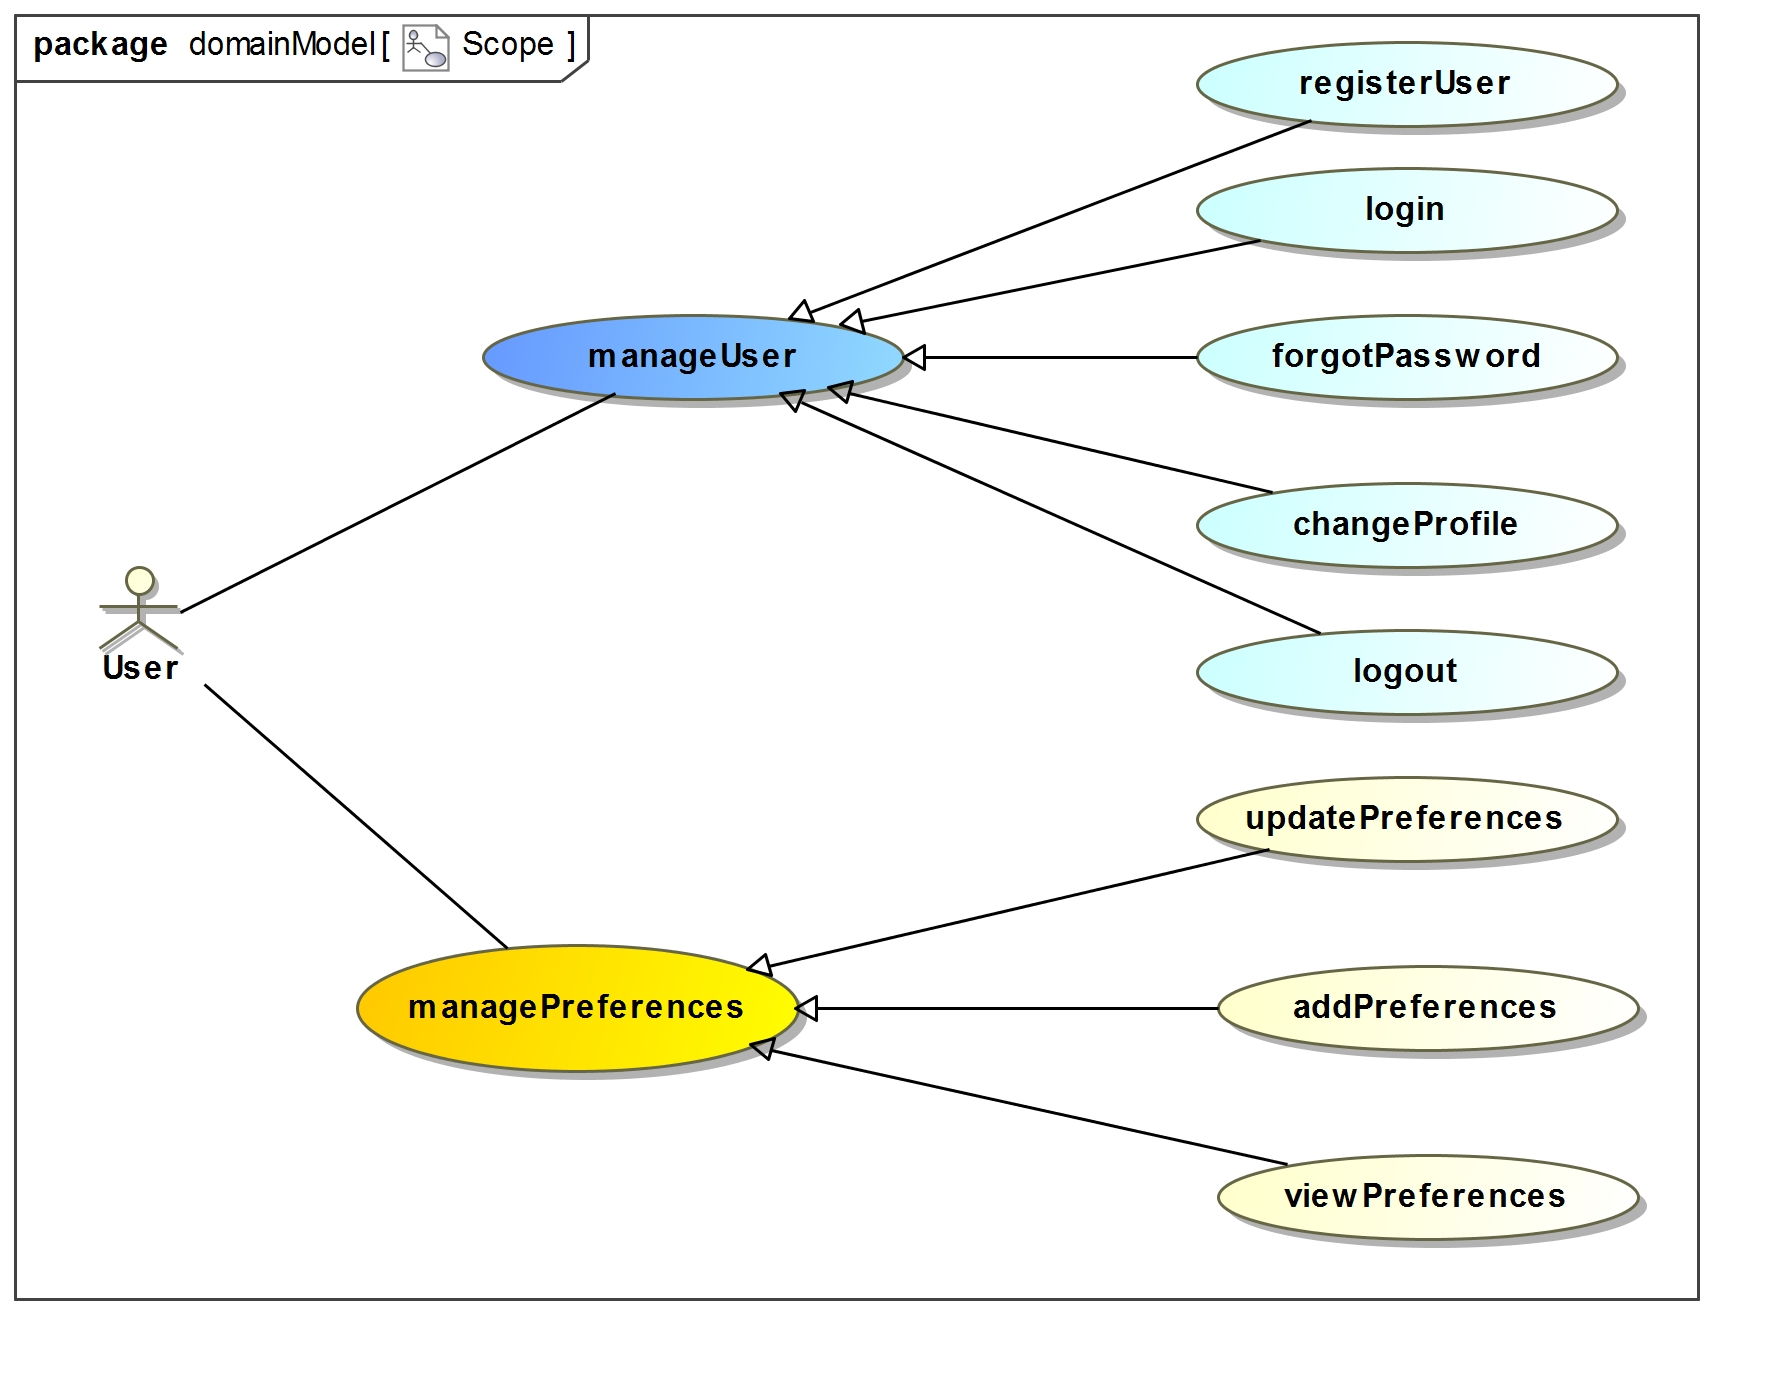
\includegraphics[width=1.0\textwidth]{../images/funcReq/UserScope.jpg}
	\caption{The scope of functionality required from the user module \label{overflow}}
\end{figure}

A user can register and login in to the system to get access to functionality such as adding,viewing and editing preferences of weather or disaster data that they would like to be at their disposal. They are also ablo to logout of the system once done.

\subsubsection{registerUser}

A user can register with the system as long as they are not already registered. Below are the service contract, activity diagram and functional requirements diagram for registerUser.

\begin{figure}[H]
	\centering
	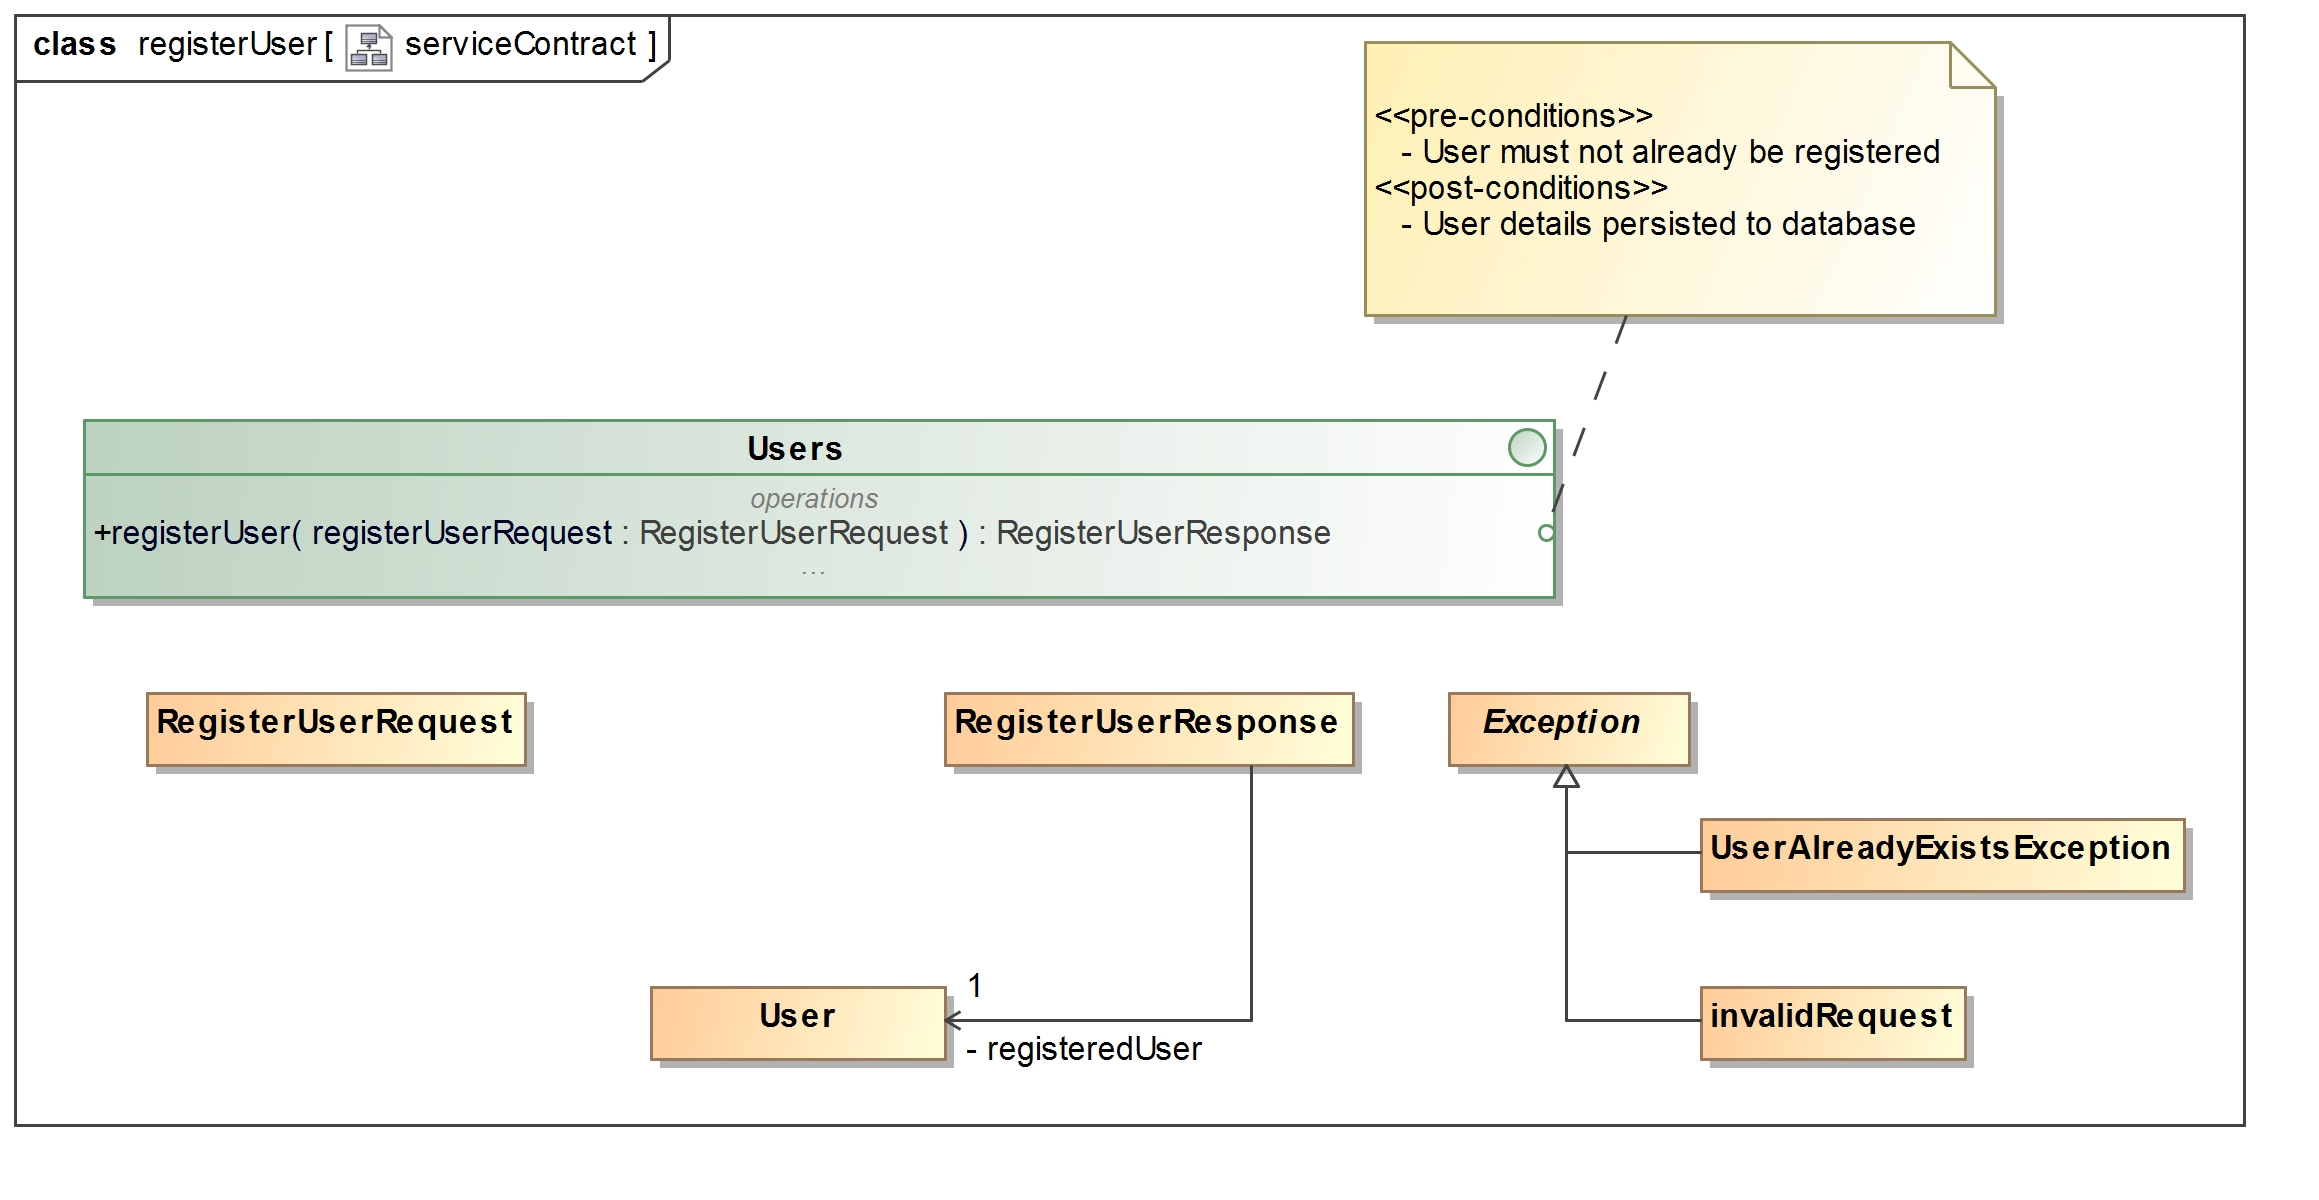
\includegraphics[width=1.0\textwidth]{../images/funcReq/registerUserServiceContract.jpg}
	\caption{The service contract for registerUser \label{overflow}}
\end{figure}

\begin{figure}[H]
	\centering
	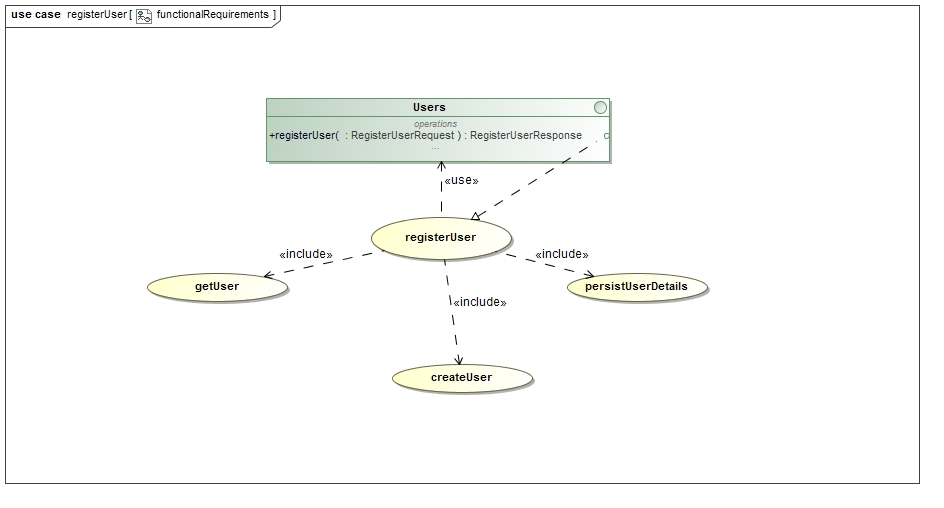
\includegraphics[width=1.0\textwidth]{../images/funcReq/registerUserFunctionalRequirements.jpg}
	\caption{The functional requirements diagram for registerUser \label{overflow}}
\end{figure}

\begin{figure}[H]
	\centering
	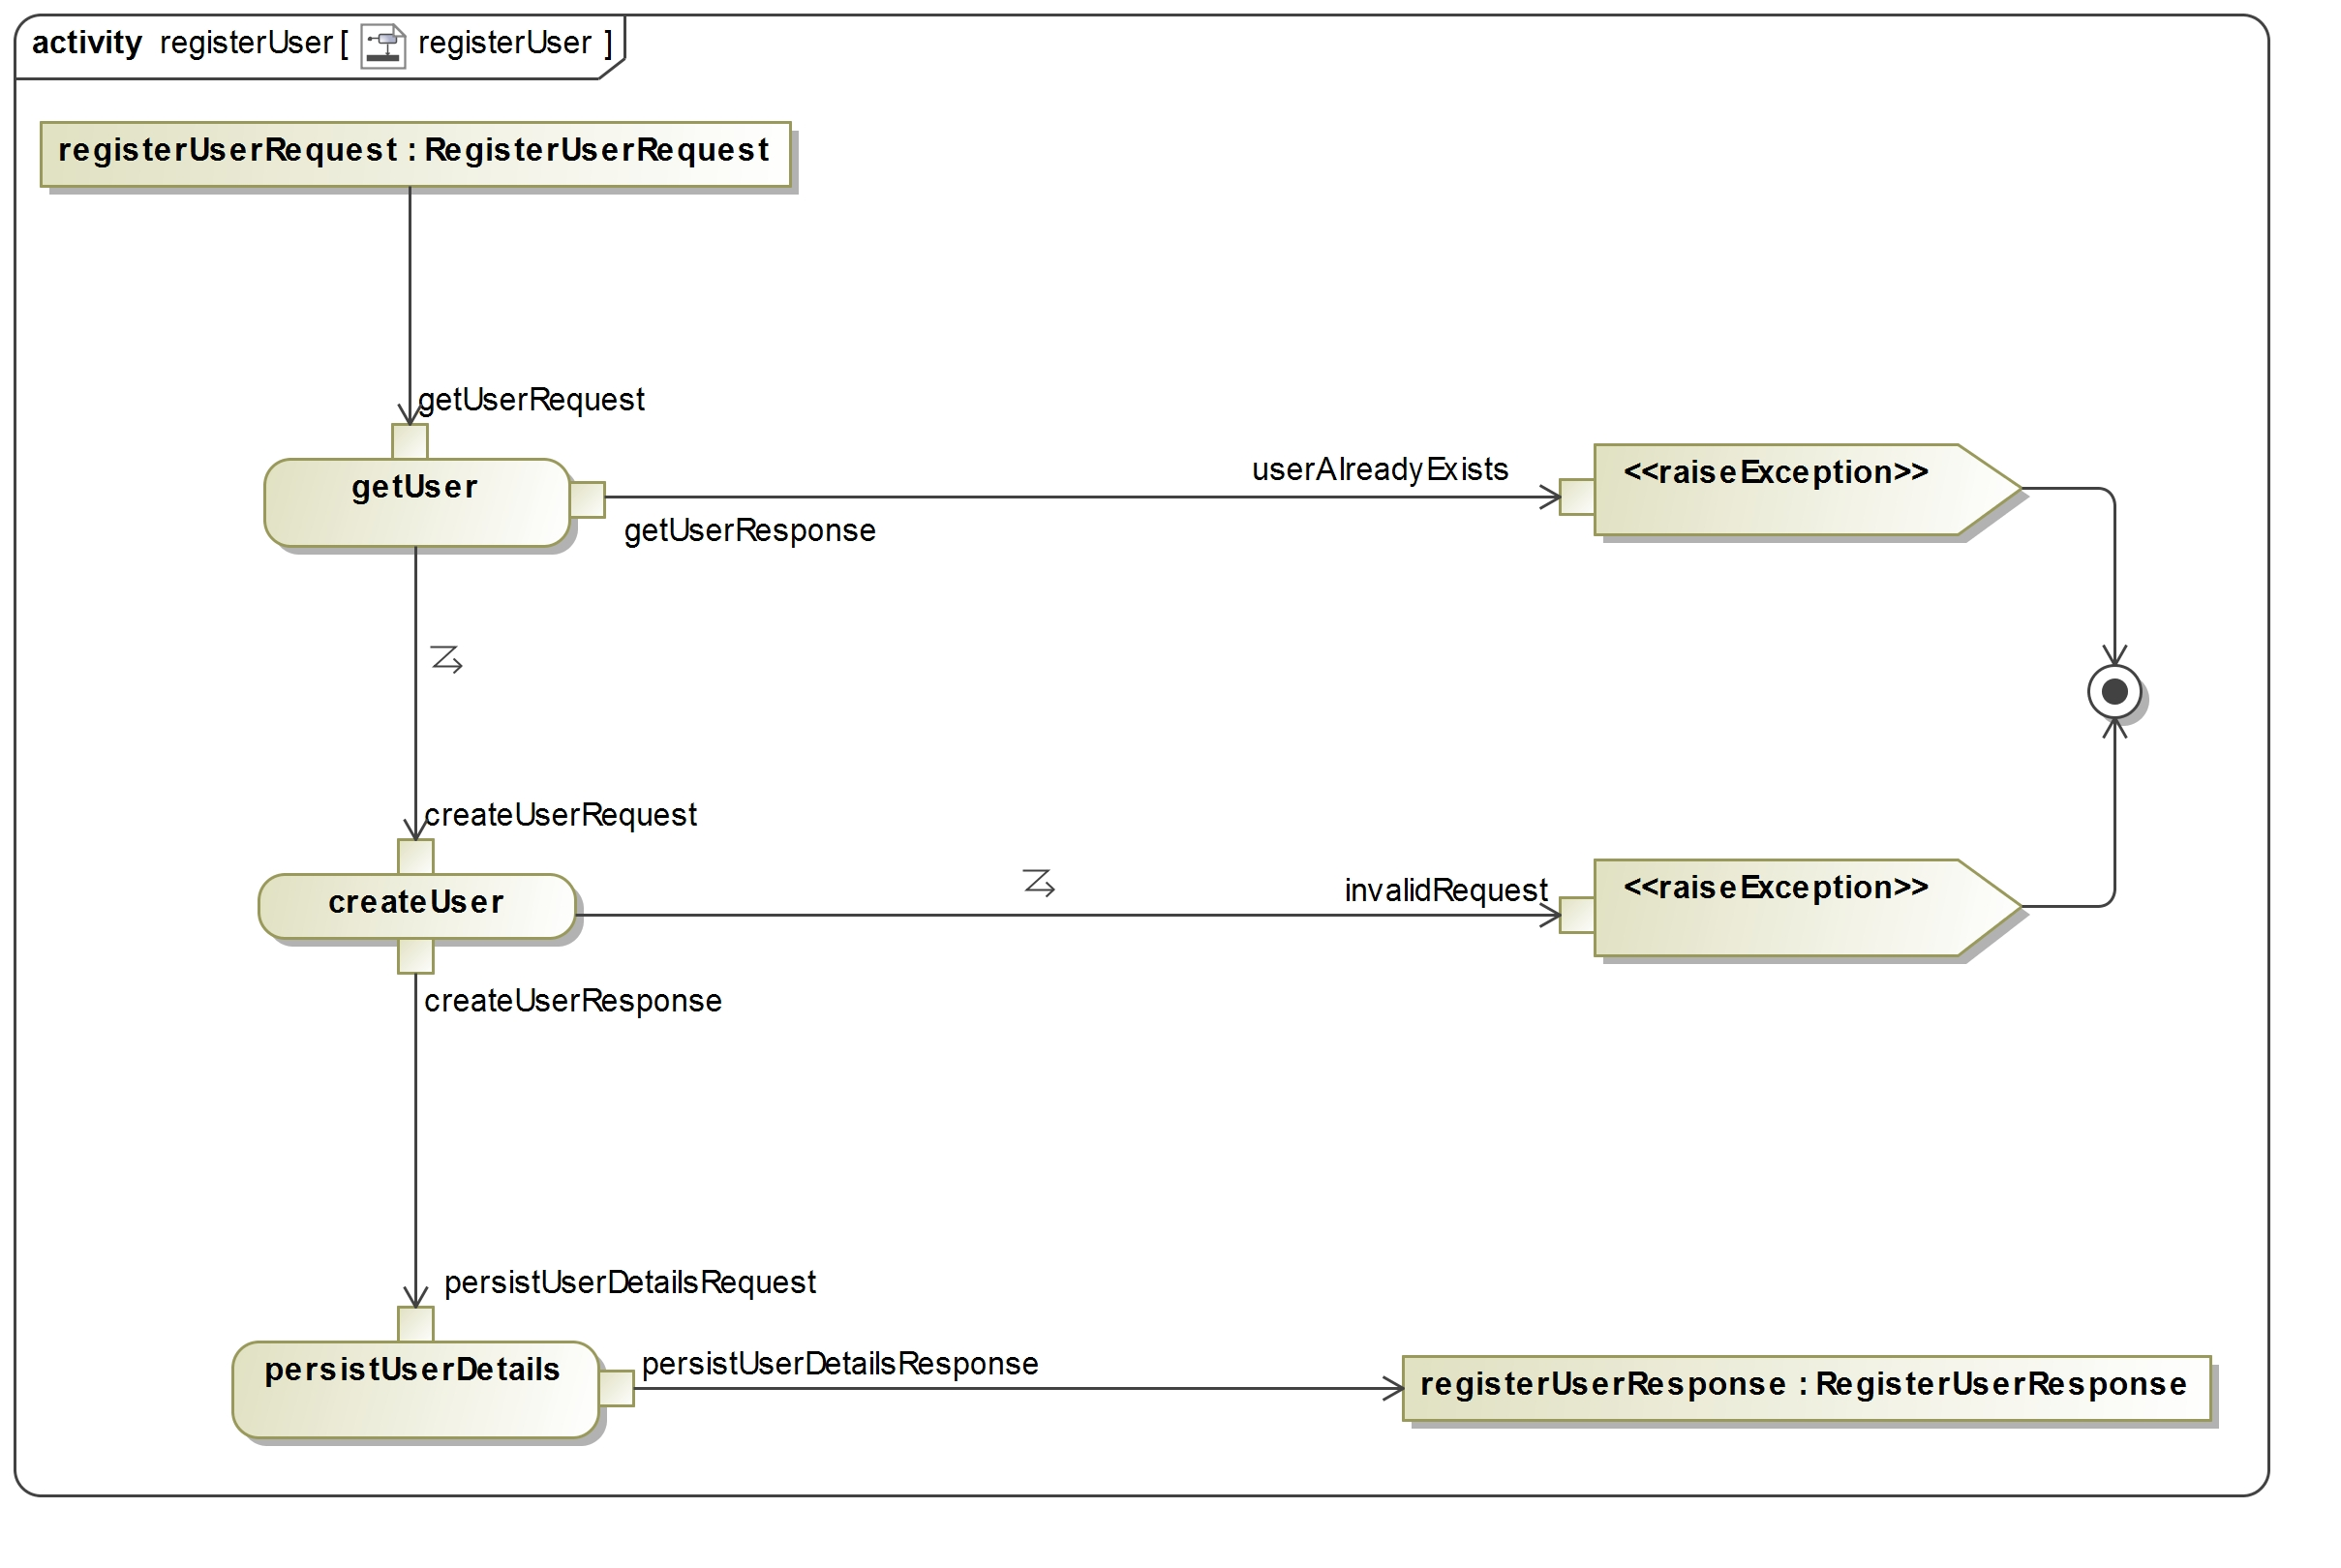
\includegraphics[width=1.0\textwidth]{../images/funcReq/registerUserActivityDiagram.jpg}
	\caption{The activity diagram for registerUser \label{overflow}}
\end{figure}

\subsubsection{login}

A registered user, given that they provide correct details to authenicate them, is able to access functionality such as adding and editing weather and disaster prefences once logged in. Below are the service contract, activity diagram and functional requirements diagram for login.

\begin{figure}[H]
	\centering
	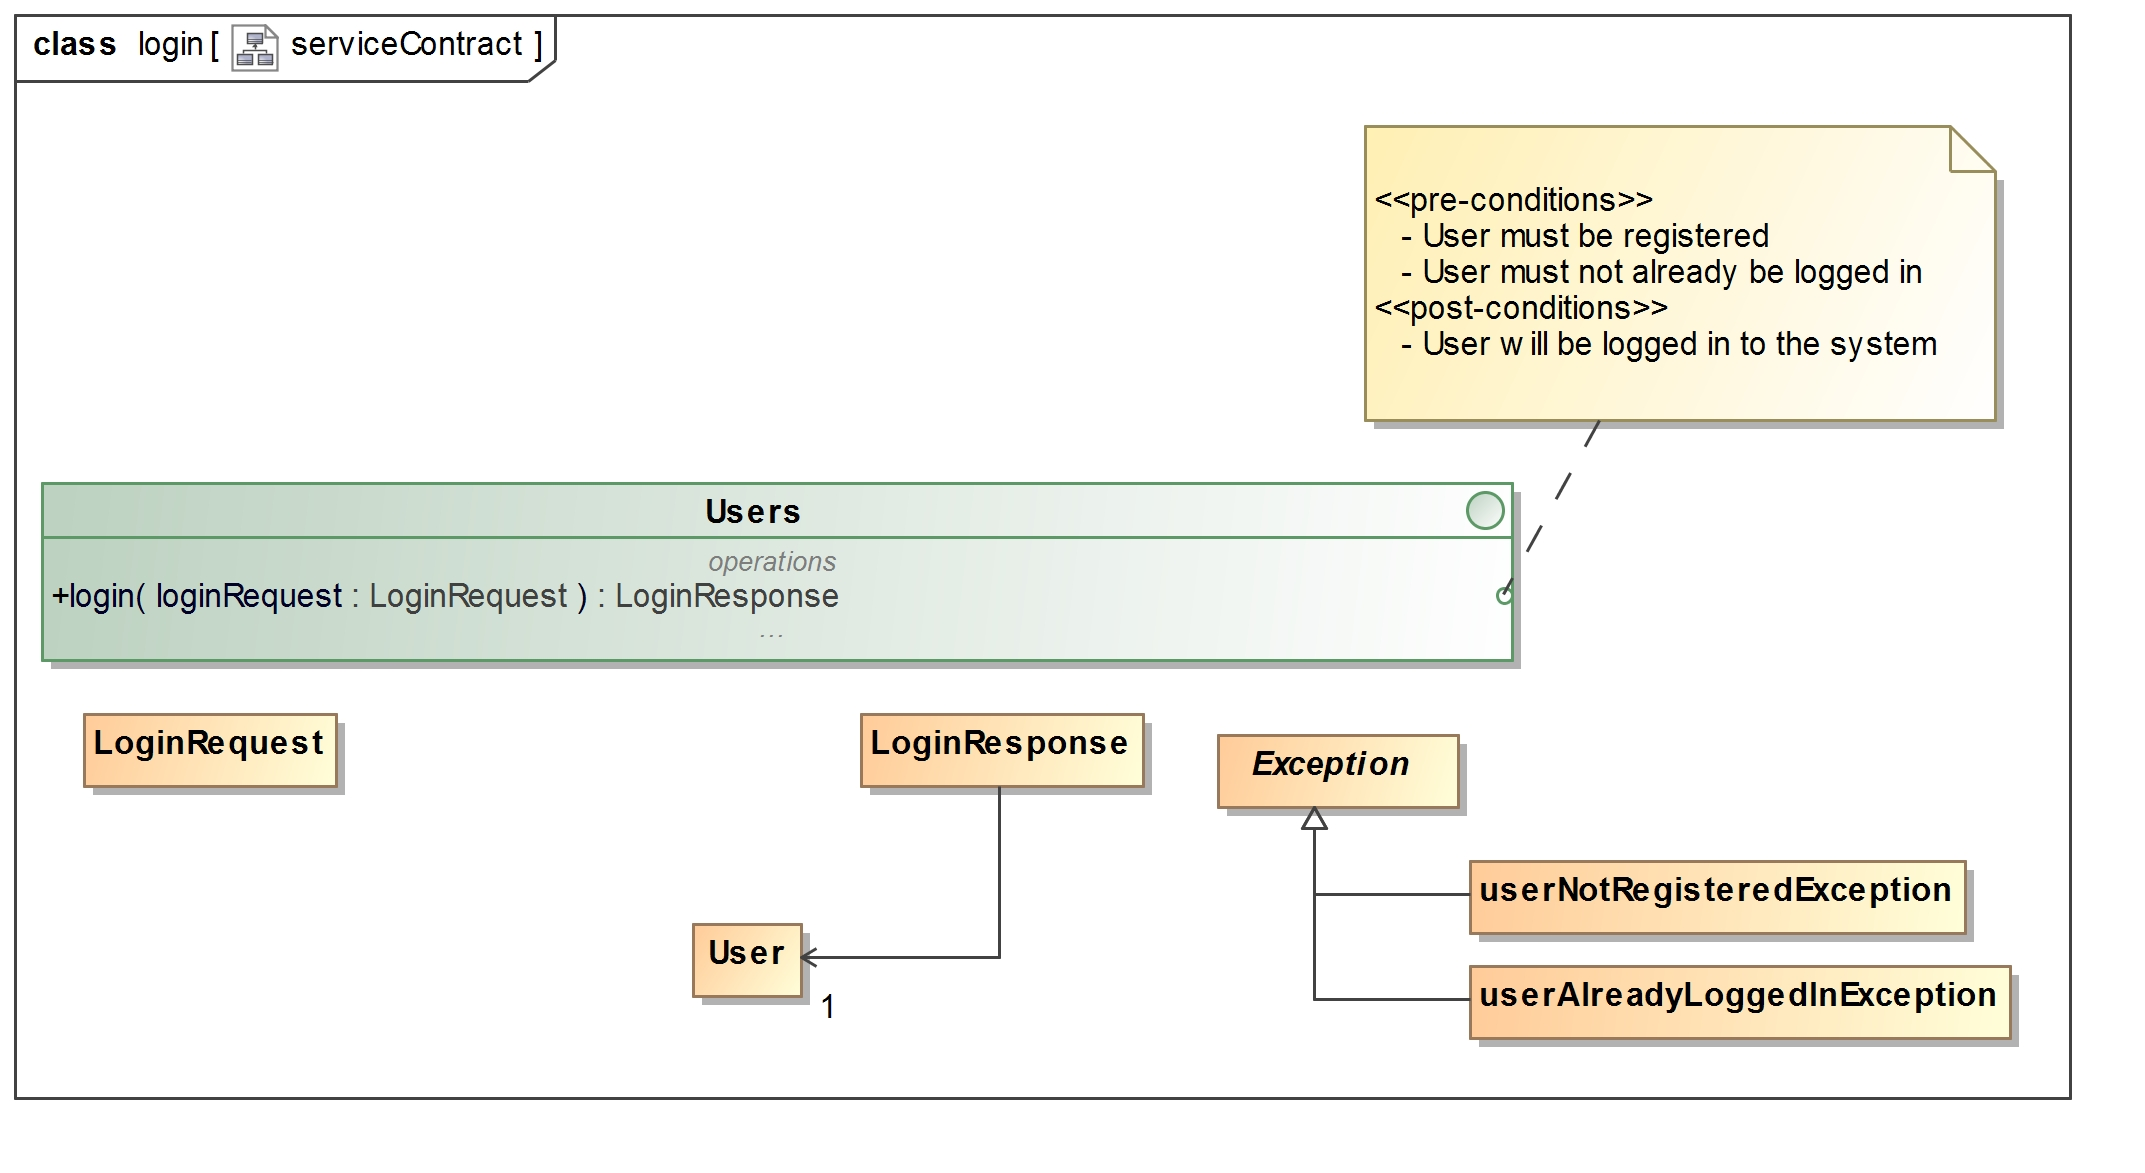
\includegraphics[width=1.0\textwidth]{../images/funcReq/loginServiceContract.jpg}
	\caption{The service contract for login \label{overflow}}
\end{figure}

\begin{figure}[H]
	\centering
	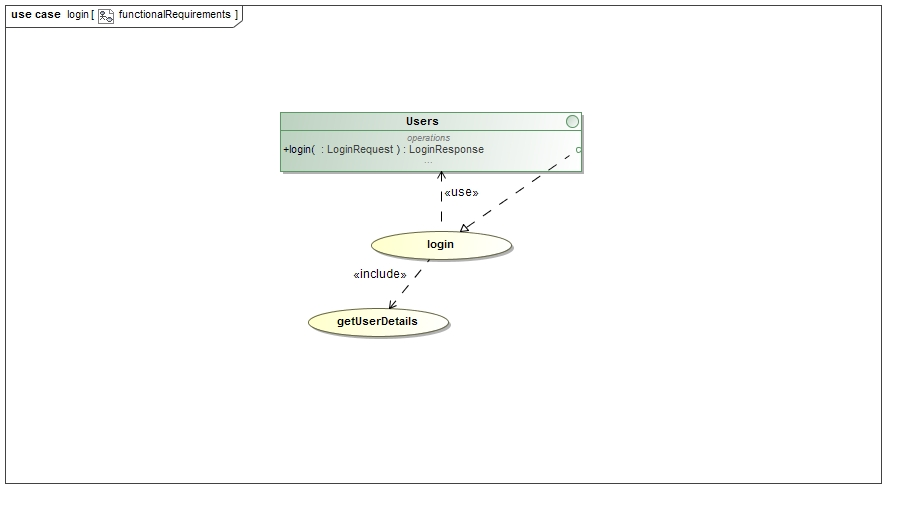
\includegraphics[width=1.0\textwidth]{../images/funcReq/loginFunctionalRequirements.jpg}
	\caption{The functional requirements diagram for login \label{overflow}}
\end{figure}

\begin{figure}[H]
	\centering
	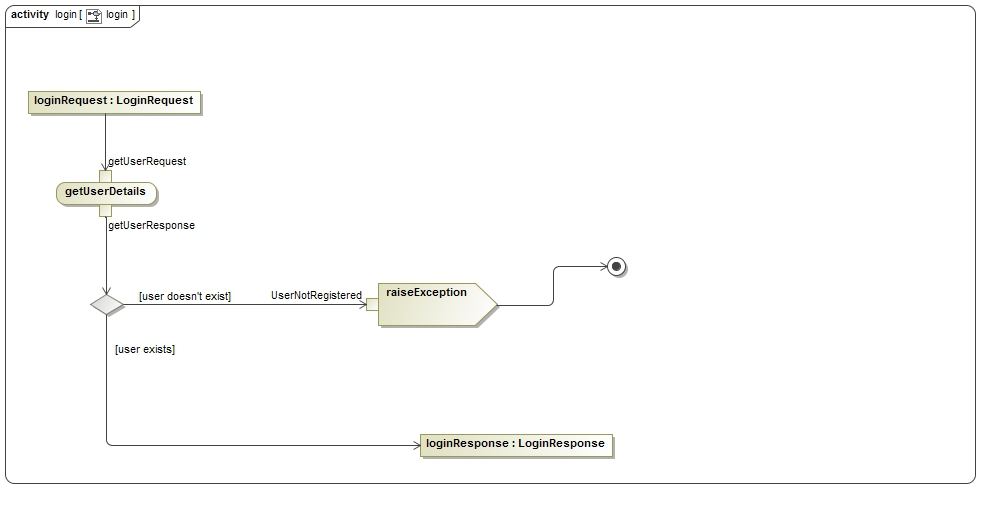
\includegraphics[width=1.0\textwidth]{../images/funcReq/loginActivityDiagram.jpg}
	\caption{The activity diagram for login \label{overflow}}
\end{figure}

\subsubsection{logout}

A user, given that they are logged in to the system, is able to logout of the system once done. Below are the service contract, activity diagram and functional requirements diagram for logout.

\begin{figure}[H]
	\centering
	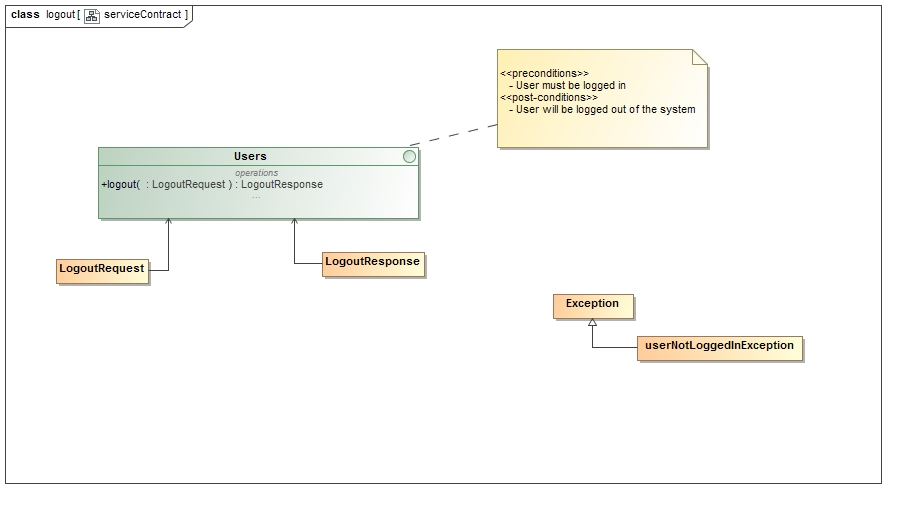
\includegraphics[width=1.0\textwidth]{../images/funcReq/logoutServiceContract.jpg}
	\caption{The service contract for logout \label{overflow}}
\end{figure}

\begin{figure}[H]
	\centering
	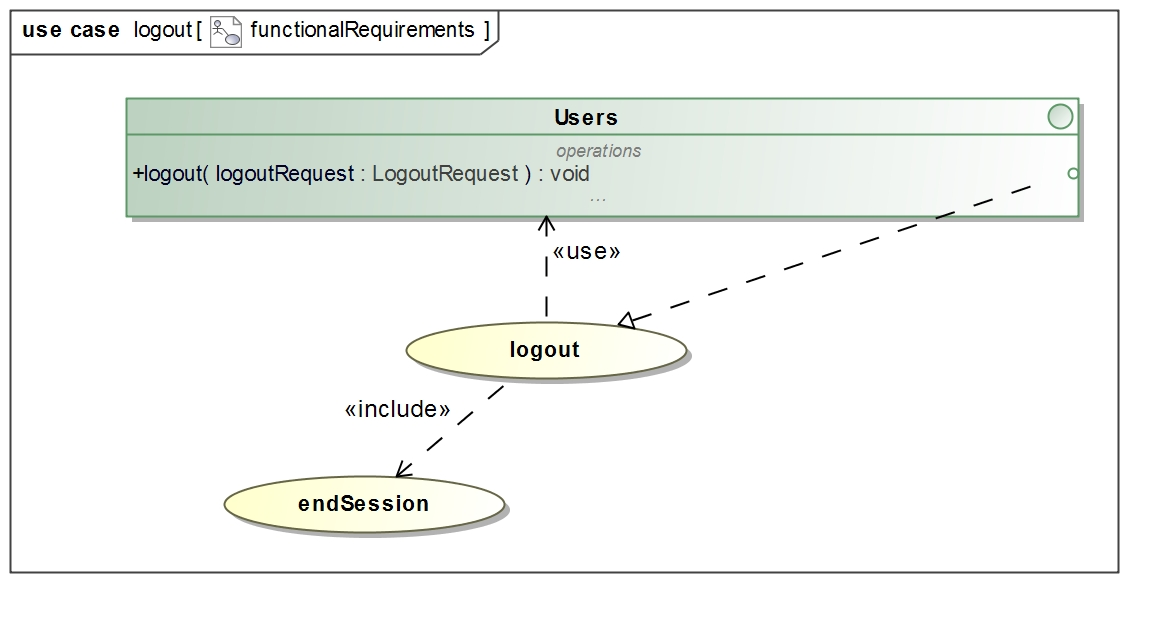
\includegraphics[width=1.0\textwidth]{../images/funcReq/logoutFunctionalRequirements.jpg}
	\caption{The functional requirements diagram for logout \label{overflow}}
\end{figure}

\begin{figure}[H]
	\centering
	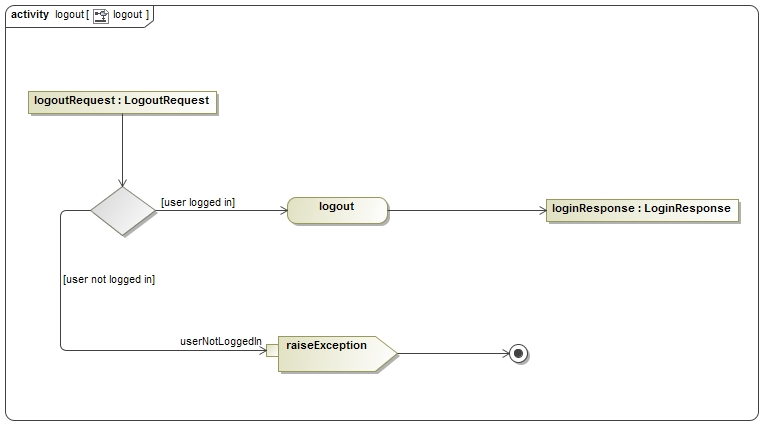
\includegraphics[width=1.0\textwidth]{../images/funcReq/logoutActivityDiagram.jpg}
	\caption{The activity diagram for logout \label{overflow}}
\end{figure}

\subsubsection{addPrefences}
\subsubsection{editPrefences}
\subsubsection{viewPrefences}
 
			
	\section{Open Issues}
	There are no issues
	
	\end{document}
